\documentclass[13pt,a4paper]{report}
\usepackage[utf8]{inputenc}
% \usepackage[english]{babel}
\usepackage{titlesec, blindtext, color}
\usepackage[table,xcdraw]{xcolor}
\usepackage{algorithm}
\usepackage{algpseudocode}
\usepackage{amsmath}
\usepackage{amssymb}
\usepackage{amsthm}
\usepackage{graphicx}
\usepackage{lmodern}
\usepackage[font=large,labelfont=bf]{caption} % Required for specifying captions to tables and figures
\usepackage[unicode]{hyperref}
\hypersetup{
colorlinks = false,
linkbordercolor = {white}
}
\usepackage[left=3cm,right=2cm,top=2.5cm,bottom=3cm]{geometry}
\usepackage{tikz}
\usetikzlibrary{calc}
\usepackage{float}
\usepackage{afterpage}
\usepackage{multirow}
\usepackage{sectsty}
\usepackage{xcolor}


\usepackage{booktabs}
\usepackage{scrextend}
\usepackage{enumerate}
\usepackage{tocloft,calc}
\usepackage{listings}

\title{Document}
\author{LTA}

\definecolor{gray75}{gray}{0.75}
\newcommand{\hsp}{\hspace{6pt}}
\titleformat{\chapter}[hang]{\small\bfseries}{\thechapter\hsp\textcolor{gray75}{|}\hsp}{0pt}{\Huge\bfseries}

\setlength{\parindent}{1cm}
% \usepackage{indentfirst}    
\setlength{\parskip}{6pt}
\chapterfont{\centering}
\renewcommand{\baselinestretch}{1.3} %format distance between lines

\usepackage{subcaption}
\usepackage{bm}
\usepackage[para]{footmisc}
\usepackage{amsfonts}
\usepackage{pdfpages}
\usepackage{xspace}


\usepackage{frontespizio}
\usepackage{perpage}
\MakePerPage{footnote}
\usepackage{longtable}
% format titile chapter section ...
\titleformat{\chapter}[display]
{\raggedright\large}
{\MakeUppercase{\chaptertitlename}~\thechapter}
{0pt}
{\vspace{2\baselineskip}\bfseries\huge}

% \titleformat*{\section}{\normalfont \Large}
% \titleformat*{\subsection}{\normalfont \large}
\sectionfont{\fontsize{15}{15}\selectfont}
\subsectionfont{\fontsize{13}{15}\selectfont}

\usepackage{biblatex}
\addbibresource{reference.bib}

\begin{document}

\begin{titlepage}
	%doubleshot titlepage's border
	\begin{tikzpicture}[overlay,remember picture]
		\draw [line width=0.8mm]
		($ (current page.north west) + (2.9cm,-2.4cm) $)
		rectangle
		($ (current page.south east) + (-1.9cm,2.9cm) $);
		\draw [line width=0.2mm]
		($ (current page.north west) + (3cm,-2.5cm) $)
		rectangle
		($ (current page.south east) + (-2cm,3cm) $);
	\end{tikzpicture}

	\begin{center}
		{\fontsize{12}{1.3}\selectfont \textbf{VIETNAM NATIONAL UNIVERSITY, HANOI\\UNIVERSITY OF ENGINEERING AND TECHNOLOGY}}

		\vspace{1.0cm}

		% \includegraphics[trim=.5cm .5cm .5cm .5cm, clip, scale=0.35]{Logo_UET}%uet's logo
		
\includegraphics[clip, scale=0.15]{overview/uet.png}

		\vspace{0.5cm}

		{\fontsize{14}{1.3}\selectfont \textbf{Le Tuan Anh}}

		\vspace{1.5cm}

		{\fontsize{18pt}{18.8pt}\selectfont \textbf{OPTIMIZE CNF ENCODING FOR ITEMSET MINING TASKS}}

		\vspace{1.75cm}

		{\fontsize{14}{1.3}\selectfont \textbf{Major: Computer Science}}

		\vfill

		{\fontsize{12}{1.3}\selectfont \textbf{HA NOI - 2024}}
	\end{center}
\end{titlepage}
\begin{titlepage}
    %doubleshot titlepage's border
    \begin{tikzpicture}[overlay,remember picture]
        \draw [line width=0.8mm]
        ($ (current page.north west) + (2.9cm,-2.4cm) $)
        rectangle
        ($ (current page.south east) + (-1.9cm,2.9cm) $);
        \draw [line width=0.2mm]
        ($ (current page.north west) + (3cm,-2.5cm) $)
        rectangle
        ($ (current page.south east) + (-2cm,3cm) $);
    \end{tikzpicture}

    \begin{center}
        {\fontsize{12}{1.3}\selectfont \textbf{VIETNAM NATIONAL UNIVERSITY, HANOI\\UNIVERSITY OF ENGINEERING AND TECHNOLOGY}}

        \vspace{1.55cm}

        {\fontsize{14}{1.3}\selectfont \textbf{Le Tuan Anh}}

        \vspace{1.5cm}

        {\fontsize{18pt}{18.8pt}\selectfont \textbf{OPTIMIZE CNF ENCODING FOR ITEMSET MINING TASKS}}

        \vspace{2.5cm}

        {\fontsize{14}{1.3}\selectfont \textbf{Major: Computer Science}}
        \vspace{2.0cm}
        \begin{flushleft} \hspace*{0.2cm} \fontsize{14}{1.3} \hspace*{0.5cm}\textbf{Supervisor: Dr. To Van Khanh} \end{flushleft}


        \vfill

        {\fontsize{12}{1.3}\selectfont \textbf{HA NOI - 2024}}
    \end{center}
\end{titlepage}
\pagenumbering{roman}
\chapter*{ABSTRACT}
\addcontentsline{toc}{chapter}{ABSTRACT}
\fontsize{13}{15}\selectfont

\textbf{Summary:} In this thesis, we apply the "Sequential Counter Encoding" method to optimize itemset mining tasks. This method has been proven effective in optimizing the search process for itemsets in data. By utilizing "Sequential Counter Encoding" we aim to enhance the performance of itemset mining algorithms while minimizing processing time.

We conduct a series of experiments on real-world datasets to evaluate the performance of the applied method. Experimental results demonstrate a significant improvement in accuracy and efficiency compared to traditional methods. The application of this method not only enhances the performance of data mining processes but also opens up potential applications for similar problems in the field of data science and information retrieval.

\textbf{\textit{Keywords: }} \textit{SAT, SAT Encoding, Sequential Counter Encoding, Itemset Mining Tasks}
\chapter*{ACKNOWLEDGEMENT}
\addcontentsline{toc}{chapter}{ACKNOWLEDGEMENT}
\fontsize{13}{15}\selectfont

First of all, I would like to express my deepest gratitude to Lecturers, Dr. To Van Khanh and Dr. Luong Thanh Nhan, who wholeheartedly guided, guided, encouraged, and helped me throughout the course of this thesis.

I would like to thank the teachers in the Faculty of Information Technology as well as the University of Engineering and Technology - Vietnam National University, Hanoi, for creating conditions for me to study in a good environment and for teaching me the best things to do. Knowledge is especially important for me to continue to study and work in the future.

I especially express my gratitude to my family who have always been a solid support to help and support me in every journey.
Finally, I would also like to thank the members of the K65CA-CLC2 class, my friends in the course, and the siblings inside and outside the school who have been with me to study and practice and help each other throughout four years university.

Thank you sincerely!


\vspace{2cm}
\begin{flushright}
    Le Tuan Anh\hspace*{1.3cm}
\end{flushright}
\chapter*{AUTHORSHIP}
\addcontentsline{toc}{chapter}{AUTHORSHIP}
\fontsize{13}{15}\selectfont

I hereby declare that the thesis "OPTIMIZE CNF ENCODING FOR ITEMSET
MINING TASKS" is done by me and has never been submitted as a report for Graduation Thesis at University of Engineering and Technology - Vietnam National University, Hanoi, or any other university. All content in this thesis is written by me and has not been copied from any source, nor is the work of others used without specific citation.
I also warrant that the source code is my development and does not copy the source code of any other person.
If wrong, I would like to take full responsibility according to the regulations of University of Engineering and Technology - Vietnam National University, Hanoi.

\vspace{0.5cm}

\begin{flushright}
    Ha Noi, May 26 2024 \par
    Student\hspace*{0.8cm}\par
    \vspace{2.5cm}
    Le Tuan Anh\par
\end{flushright}
\chapter*{SUPERVISOR’S APPROVAL}
\addcontentsline{toc}{chapter}{SUPERVISOR’S APPROVAL}
\fontsize{13}{15}\selectfont

I hereby approve that the thesis in its current form is ready for committee examination as a requirement for the Bachelor of Computer Science degree at the University of Engineering and Technology.

\vspace{1cm}

\begin{flushright}
    Ha Noi, May 26 2024 \par
    Supervisor\hspace*{0.8cm}\par
    \vspace{2.5cm}
    Dr. To Van Khanh\par
\end{flushright}
% \pagenumbering{gobble}
\tableofcontents
% \newpage
\listoffigures
% \newpage
% \listoftables
% \nomenclature{SAT}{Satisfiability}
% \nomenclature{UNSAT}{Unsatisfiability}
% \nomenclature{CNF}{Conjunctive Normal Form}
% \nomenclature{ALO}{At Least One}
% \nomenclature{AMO}{At Most One}
% \printnomenclature

\chapter*{ABBREVIATIONS}
\addcontentsline{toc}{chapter}{ABBREVIATIONS}

\begin{table}[htbp]
    \raggedright
    \begin{tabular}{ll}
        \\
        FIM   & Frequent Itemset Mining                    \\
        SEE   & Sequential Encounter Encoding              \\
        SAT   & Satisfiability                             \\
        UNSAT & Unsatisfiability                           \\
        CNF   & Conjunctive Normal Form                    \\
        ALO   & At Least One                               \\
        AMO   & At Most One                                \\
        ALK   & At Least k                                 \\
        AMK   & At Most k                                  \\
        FIMI  & Frequent Itemset Mining Dataset Repository \\
        CP4IM & Constraint Programming for Itemset Mining  \\
    \end{tabular}
\end{table}
\chapter*{PREFACE}
\addcontentsline{toc}{chapter}{PREFACE}
\fontsize{13}{15}\selectfont

Itemset mining, a fundamental task in data mining, plays a pivotal role in discovering meaningful patterns from large datasets. It involves identifying sets of items that frequently co-occur together within transactions, providing valuable insights into associations and correlations among items.

In this thesis, we delve into the realm of itemset mining and its crucial importance in various domains such as market basket analysis, bioinformatics, and web usage mining. We explore the significance of itemset mining in uncovering hidden patterns, aiding decision-making processes, and enhancing business strategies.

Furthermore, we aim to optimize the itemset mining process by leveraging the Sequential Encounter Encoding method for SAT encoding. This innovative approach offers a novel perspective on encoding itemset mining problems into Boolean satisfiability (SAT) instances, paving the way for efficient and scalable solutions.

The subsequent chapters of this thesis are structured as follows:

\textbf{Chapter 1}: This chapter serves as an introduction to itemset mining tasks and SAT encoding. It elucidates the fundamental concepts, terminology, and real-world applications associated with these fields.

\textbf{Chapter 2}: We delve into the construction of base constraints for itemset mining problems and their encoding into SAT. This includes an exploration of the process of deriving constraints from standard itemset mining algorithms, along with an analysis of their limitations.

\textbf{Chapter 3}: Here, we discuss the Sequential Encounter Encoding method as a novel approach to encoding itemset mining problems into SAT instances. We delve into the intricacies of this encoding technique and highlight its advantages over traditional methods.

\textbf{Chapter 4}: This chapter presents the results of experimental evaluations conducted on both synthetic and real-world datasets. We compare the performance of the Sequential Encounter Encoding method with existing approaches to showcase its efficacy and scalability.

\textbf{Chapter 5}: Finally, we conclude our findings, summarizing the contributions of this research and discussing potential avenues for future exploration in the field of itemset mining and SAT encoding.

Through this thesis, we aim to contribute to the advancement of itemset mining techniques and facilitate the development of more efficient algorithms for pattern discovery in large datasets.

\pagenumbering{arabic}
\fontsize{13}{15}\selectfont

\chapter{Introduction}
This chapter will focuses on introducing the itemset mining tasks and SAT encoding, encompassing their concepts, related terms, and applications.
\section{Itemset Mining Tasks}
\subsection{Overview}
Frequent item sets are a key technique in the realm of data mining\cite{FIM_geeksforgeeks},
specifically aimed at uncovering relationships among different items.
The essence of association rule mining lies in identifying those item relationships that occur frequently together in the dataset.

In simpler terms, imagine a "frequent itemset" as a group of items that tend to show up in unison across various data entries. We utilize a specific measure called 'support count' to gauge the regularity of these itemset occurrences. The support count essentially quantifies the number of times a particular combination of items appears within the dataset's entries or transactions.

The practical aim here is to pinpoint those itemsets that reach or surpass a predetermined threshold of occurrence, known as the minimum support. By identifying these itemsets, we can infer patterns of frequency within the dataset's transactions or records.

For example, with a dataset of transactions from a retail store
\begin{table}[H]
    \centering
    \caption{Example of a dataset of transactions}
    \label{tab:example_dataset_in_real}
    \begin{tabular}{|c|l|}
        \hline
        \textbf{Tid} & \textbf{Itemsets}     \\
        \hline
        1            & apple, banana, cherry \\
        2            & apple, mango          \\
        3            & apple, cherry         \\
        4            & mango, cherry         \\
        5            & apple, mango, cherry  \\
        \hline
    \end{tabular}
\end{table}

With minimum support is 3, we need to find all itemsets appearing in at least 3 transactions and return the following result:

\begin{itemize}
    \item Itemset 1: \{apple, cherry\} in transactions [1, 3, 5]
    \item Itemset 2: \{apple\} in transactions [1, 2, 3, 5]

\end{itemize}

\subsection{Applications}
Frequent itemset mining is a powerful analytic process used to examine the relationships between items in large datasets. Taking a practical example from the commercial realm, let's picture a supermarket setting.

Through the lens of frequent itemset mining, a supermarket can sift through transactional data to identify combinations of items that customers tend to purchase together regularly. This type of analysis digs deeper than observing mere coincidental purchases; it uncovers patterns that reflect a certain predictability and frequency in customer buying behavior.

For example, a pattern where bread and milk are often purchased together reflects a habitual buying behavior rather than a sporadic trend. These insights are invaluable for retailers, as they allow them to make informed decisions across various aspects of their operations.

Here's how these insights translate into real-world advantages:

Inventory Management: By understanding which itemsets are popular, retailers can better manage their inventory, ensuring that these items are always in stock and accessible to customers. This proactive approach helps avoid stock shortages and enhances the overall shopping experience.

Recommendation Systems: Retailers can implement systems that use frequent itemset data to recommend additional products to customers. For instance, if a customer selects pasta, the system might suggest accompanying it with pasta sauce and grated cheese, based on observed buying patterns. This can lead to greater customer satisfaction and increased sales.

Targeted Marketing: The knowledge of which items are often bought together allows retailers to tailor their marketing efforts. Promotions can be strategized to bundle popular itemsets, attracting customers and encouraging them to buy more.

In essence, frequent itemset mining is a strategic tool in the business intelligence arsenal. It empowers businesses with deep insights into consumer purchasing trends, facilitating data-driven strategies that foster growth and enhance customer engagement.

\section{SAT Encoding}
\subsection{Concept}
The concept of SAT, also known as the Boolean Satisfiability problem,
is a computer science problem aimed at determining the satisfiability of a propositional logic formula.

\begin{flushleft}
    \textbf{Input}: A propositional logic formula, typically represented in Conjunctive Normal Form (CNF).
\end{flushleft}

\begin{flushleft}
    \textbf{Output}:
\end{flushleft}
\begin{itemize}
    \item SAT (Satisfiable): If there exists a truth value assignment (true/false) to the
          logical variables that makes the original propositional logic formula evaluate to true.
    \item UNSAT (Unsatisfiable): If every truth value assignment (true/false) to the
          logical variables results in the original propositional logic formula evaluating to false.
\end{itemize}

\subsection{Encoding}
SAT Encoding is a method in which certain problems can be solved by transforming
them into SAT problems: representing problems using propositional logic formulas and
applying SAT Solvers to solve these propositional logic formulas.

\begin{figure}
    \centering
    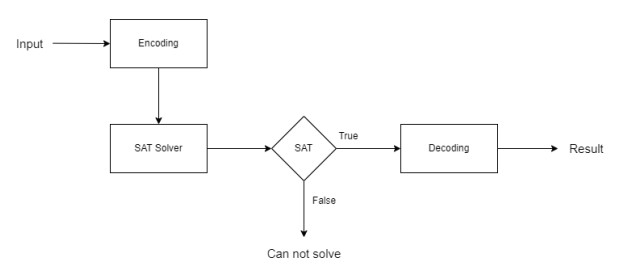
\includegraphics[width=0.9\textwidth]{chapter1/image/flow_sat.jpg}
    \caption{SAT Encoding Process}
    \label{fig:sat_encoding_process}
\end{figure}

A problem solved using SAT Encoding follows the following steps: First, identify the
input data or the problem's input that needs to be solved. The Encoding module then
takes this input data, defines the rules, and encodes these rules into Conjunctive Normal
Form (CNF) logical formulas, producing an output file containing the number of
variables, the number of clauses, and the CNF formulas. The SAT Solver takes the
output file from the Encoding module as input, processes the expressions, and generates
the output result. The output result can be SAT if the SAT Solver finds a dataset
satisfying the CNF formulas, or UNSAT if it fails to find any dataset. If the result is
SAT, the SAT Solver provides another file containing the corresponding dataset it
found. From the discovered dataset, the solution to the problem can be inferred, resulting
in the corresponding answer for the input data.

\subsection{SAT Solvers}
SAT Solver is a tool designed to solve the Boolean Satisfiability (SAT) problem,
determining whether a propositional logic formula is satisfiable or not. It utilizes CNF
(Conjunctive Normal Form) formulas.

In the SAT problem, we are given n Boolean variables and m clauses, where each clause
is the disjunction of a set of literals, and a literal is a variable or its negation. The aim is
to decide whether there is an interpretation of the variables that satisfies all clauses.
Currently, numerous SAT- tools can efficiently handle a large number of clauses and
variables, providing optimal results. Examples include Minisat [2], Lingeling [3],
Glucose [4], RSat [5].

SAT is proven to be NP-complete, meaning it has exponential time complexity in the
worst case scenario. Despite this, effective and scalable algorithms for SAT have been
developed in the 2000s, significantly advancing the automatic resolution of problems
with tens of thousands of variables and millions of clauses [6]. One such algorithm used
by SAT Solvers is DPLL (Davis-Putnam-Logemann-Loveland), introduced in 1961,
relying on a backtracking, exhaustive search approach.

Modern SAT-solving methods introduced in the 2000s have incorporated the Conflict
Driven Clause Learning (CDCL) algorithm alongside DPLL, enhancing the efficiency
of SAT Solvers in various domains.

Kissat is a "keep it simple and clean bare metal SAT solver" written in C.
It is a port of CaDiCaL back to C with improved data structures, better scheduling of inprocessing and optimized algorithms and implementation.
The CNF file format used by Kissat consists of the following components:

\begin{itemize}
    \item The first line specifies the number of variables and the number of clauses in the CNF file.
    \item The subsequent lines contain the CNF-formatted logical statements, represented as clauses.
\end{itemize}

\begin{center}
    \begin{verbatim}
        p cnf [number of variables] [number of clauses]
        [clauses]
    \end{verbatim}
\end{center}

\begin{flushleft}
    In this format:
\end{flushleft}
\begin{itemize}
    \item \texttt{p cnf} denotes the CNF format.
    \item \texttt{[number of variables]} denotes the count of logical variables used.
    \item \texttt{[number of clauses]} represents the number of logical clauses.
    \item \texttt{[clauses]} refers to the CNF-formatted logical statements.
\end{itemize}

For example:
\begin{center}
    \begin{verbatim}
        p cnf 3 2
        1 -2 0
        2 3 -1 0
    \end{verbatim}
\end{center}

This CNF file contains 3 variables and 2 clauses.
The first clause is \texttt{[1 -2 0]}, and the second clause is \texttt{[2 3 -1 0]}.
The \texttt{0} at the end of each clause denotes the end of the clause.
It represented as logical formulas:
\begin{center}
    $(x_1 \vee \neg x_2) \wedge (x_2 \vee x_3 \vee \neg x_1)$.
\end{center}

The SAT problem can be solved by running the Kissat SAT Solver on the CNF file.
The output will indicate whether the logical formula is satisfiable or unsatisfiable
and provide the truth value assignments for the logical variables with format:
\begin{center}
    \begin{verbatim}
        s [status]
        v [variable assignments]
    \end{verbatim}
\end{center}

For this given CNF file, the output will be:
\begin{center}
    \begin{verbatim}
        s SAT
        v 1 -2 -3
    \end{verbatim}
\end{center}

But it is only one of the possible solutions, there are many other solutions that satisfy the CNF formula.
To find all solutions, we need to append the solution found as a clause and run the SAT Solver again.
This process is repeated until the SAT Solver returns UNSAT, indicating that all solutions have been found.

\subsection{Applications}
In addition to SAT Encoding, SAT is utilized in various fields of information
technology. Notable areas include: In formal methods, SAT is used for hardware model
testing, software model testing, and test pattern generation. In the field of artificial
intelligence, SAT is employed for planning, knowledge representation problems, and in
intelligent games. In the realm of automated design, SAT is applied for equivalence
checking, delay computation, error detection, and more.
\section{Technical background}
\subsection{Propositional Expression}
Propositional logic formulas or propositional expressions are constructed from variables
and logical operators AND (conjunction), OR (disjunction), NOT (negation), and
parentheses.

\textbf{Proposition}: Each statement that can be either true or false is called a proposition,
denoted by letters such as P, Q, R, ...

\textbf{Negation}

The negation (NOT) of a proposition P is denoted by $\lnot$ P. The negation
is true when P is false.

Truth table:
\begin{table}[H]
    \centering
    \caption{Truth table of negation (NOT)}
    \label{tab:truth_table_negation}v
    \begin{tabular}{|c|c|}
        \hline
        P & $\lnot$ P \\
        \hline
        T & F         \\
        F & T         \\
        \hline
    \end{tabular}
\end{table}

\textbf{Conjunction}

The conjunction (AND) of two propositions P and Q is denoted by P
$\land$ Q. The conjunction is true only when both P and Q are true.

Truth table:
\begin{table}[H]
    \centering
    \caption{Truth table of conjunction (AND)}
    \label{tab:truth_table_conjunction}
    \begin{tabular}{|c|c|c|}
        \hline
        P & Q & P $\land$ Q \\
        \hline
        T & T & T           \\
        T & F & F           \\
        F & T & F           \\
        F & F & F           \\
        \hline
    \end{tabular}
\end{table}

\textbf{Disjunction}

The disjunction (OR) of two propositions P and Q is denoted by P $\lor$ Q.
The disjunction is true when at least one of P and Q is true.

Truth table:
\begin{table}[H]
    \centering
    \caption{Truth table of disjunction (OR)}
    \label{tab:truth_table_disjunction}
    \begin{tabular}{|c|c|c|}
        \hline
        P & Q & P $\lor$ Q \\
        \hline
        T & T & T          \\
        T & F & T          \\
        F & T & T          \\
        F & F & F          \\
        \hline
    \end{tabular}
\end{table}

\textbf{Implication}

The implication of two propositions P and Q is denoted by P $\rightarrow$ Q.
The implication is false only when P is true and Q is false.

Truth table:
\begin{table}[H]
    \centering
    \caption{Truth table of implication}
    \label{tab:truth_table_implication}
    \begin{tabular}{|c|c|c|}
        \hline
        P & Q & P $\rightarrow$ Q \\
        \hline
        T & T & T                 \\
        T & F & F                 \\
        F & T & T                 \\
        F & F & T                 \\
        \hline
    \end{tabular}
\end{table}

\textbf{Biconditional}

The biconditional of two propositions P and Q is denoted by P $\leftrightarrow$ Q.
The biconditional is true when both P and Q have the same truth value.

Truth table:
\begin{table}[H]
    \centering
    \caption{Truth table of biconditional}
    \label{tab:truth_table_biconditional}
    \begin{tabular}{|c|c|c|}
        \hline
        P & Q & P $\leftrightarrow$ Q \\
        \hline
        T & T & T                     \\
        T & F & F                     \\
        F & T & F                     \\
        F & F & T                     \\
        \hline
    \end{tabular}
\end{table}

\subsection{Conjunction Normal Form (CNF)}

A propositional formula is in conjunctive normal form (CNF) if it is a conjunction of clauses, where each clause is a disjunction of literals. A literal is a propositional variable or its negation.
The standard form of CNF is
\begin{equation*}
    (P_1 \lor P_2 \lor ... \lor P_n)_1 \land ... \land (Q_1 \lor Q_2 \lor ... \lor Q_m)_p \quad n,m,p \geq 1
\end{equation*}

Sample truth table (only for P and Q and R):
\begin{table}[H]
    \centering
    \caption{Truth table of CNF}
    \label{tab:truth_table_cnf}
    \begin{tabular}{|c|c|c|c|}
        \hline
        P & Q & R & (P $\land$ Q) $\land$ R \\
        \hline
        T & T & T & T                       \\
        T & T & F & F                       \\
        T & F & T & F                       \\
        T & F & F & F                       \\
        F & T & T & F                       \\
        F & T & F & F                       \\
        F & F & T & F                       \\
        F & F & F & F                       \\
        \hline
    \end{tabular}
\end{table}

\subsection{Technical background of Itemset Mining}
Firstly, we establish several symbols to represent the itemset mining problem.
These symbols aid in formalizing the problem and defining key concepts.
For instance, we denote:
\begin{itemize}
    \item \textbf{$\Omega$}: a set of all items
    \item \textbf{$I$}: an itemset in $\Omega$, where $I \subseteq \Omega$
    \item \textbf{$T_i$}: a transaction identifier. For $T_i$ = $(i,I)$
    \item \textbf{$D$}: a transaction database, where $D$ contains a set of transactions, $D = \{T_1, T_2, ..., T_n\}$
    \item \textbf{$Supp(I, D)$}: the support of itemset $I$ in database $D$, where $Supp(I, D)$ is the number of transactions in $D$ that contain $I$
\end{itemize}
For example, in table \ref{tab:example_dataset_in_real},
we can present the dataset as a transaction database $D$.

Let $a = apple, b = banana, c = cherry, d = mango$.
Then we have database transactions in binary format as shown in table \ref{tab:example_dataset_convert_to_binary}.

\begin{table}[H]
    \centering
    \caption{Sample dataset of transactions in binary format}
    \label{tab:example_dataset_convert_to_binary}
    \begin{tabular}{|c| c c c c |}
        \hline
        \textbf{Tid} & \textbf{a} & \textbf{b} & \textbf{c} & \textbf{d} \\
        \hline
        1            & 1          & 1          & 1          & 0          \\
        2            & 1          & 0          & 0          & 1          \\
        3            & 1          & 0          & 1          & 0          \\
        4            & 0          & 0          & 1          & 1          \\
        5            & 1          & 0          & 1          & 1          \\
        \hline
    \end{tabular}
\end{table}

\begin{itemize}
    \item $\Omega$ is \{apple, banana, cherry, mango\}
    \item $I$ can be \{apple\}, \{apple, mango\}, \{apple, mango, cherry\}, ...
    \item $D$ = \{(1, \{apple, banana, cherry\}), (2, \{apple, mango\}), (3, \{apple, cherry\}), (4, \{mango, cherry\}), (5, \{apple, mango, cherry\})\}
    \item $T_1$ = (1, \{apple, banana, cherry\}), $T_2$ = (2, \{apple, mango\}), $T_3$ = (3, \{apple, cherry\}),...
    \item $Supp(\{apple, cherry\}, D)$ = 3, $Supp(\{apple\}, D)$ = 4,...
\end{itemize}
Let $\lambda$ be the minimum support threshold,
the frequent itemset mining problem is to find all itemsets $I$ such that $Supp(I, D) \geq minsup$. In general, it can present by:

\begin{center}
    $FIM(D,\lambda)$ = \{I $\subseteq \Omega$ $|$ $Supp(I, D) \geq \lambda$\}
\end{center}

One of the major challenges in itemset mining is the potential exponential growth of the output, even when using condensed representations of patterns.



\chapter{SAT-based Encoding of Itemset Mining}
In this chapter, we provide a detailed walkthrough of encoding the itemset mining problem into a SAT problem.
We begin by establishing variable conventions and introducing constraints, gradually transitioning to converting these constraints into Conjunctive Normal Form (CNF) using the standard method.
Along the way, we discuss the limitations of the standard method, particularly in handling large datasets or high support thresholds.
Our goal is to equip readers with a clear understanding of the SAT encoding process for itemset mining and the challenges it entails.

\section{Base constraints}
To resolve the itemset mining problem, we using the SAT encoding approach.
In essence, SAT encoding involves the creation of variables and the imposition of constraints to represent the itemset mining problem.
These variables serve to denote the presence or absence of items within a candidate itemset and are subjected to linear inequalities to ensure the itemset's support.

In the context of a transaction database $D$ = {(1,$T_1$),...,(m,$T_m$)} and a minimum support threshold $\lambda$,
each item in the candidate itemset $X$, we denote:
\begin{itemize}
    \item $p_a$: is $true$ if the item $a$ is in the itemset $X$, otherwise $p_a = false$
    \item $q_i$: is $true$ if the transaction $T_i$ contains the itemset $X$, otherwise $q_i = false$
\end{itemize}
Alongside, a set of constraints is imposed on these variables to establish a one-to-one correspondence between the models of the resulting CNF formula and the set of itemsets.

Firstly, to capture all the transactions where the candidate itemset does not appear, we use following constraint:
\begin{equation}
    \label{eq:1}
    \bigwedge_{i=1}^{m} (q_i \leftrightarrow \bigwedge_{a \notin T_i} \neg p_a)
\end{equation}
This constraint guarantees that $q_i$ is true if and only if either all items not in $T_i$ are also not in the itemset $X$, or transaction $T_i$ contains the itemset $X$.

Constraint \ref{eq:1} can be rewritten as follows:
\begin{equation}
    \label{eq:2}
    \bigwedge_{a \in \Omega} \bigwedge_{a \notin T_i} (\neg p_a \vee \neg q_i)
\end{equation}
\begin{equation}
    \label{eq:3}
    \bigwedge_{T_i \in D} ((\bigvee_{a \notin T_i} p_a) \vee q_i)
\end{equation}


Finally, the frequency constraint, can be simply expressed as follows:
\begin{equation}
    \label{eq:4}
    \sum_{i=1}^{m} q_i \geq \lambda
\end{equation}

For example, with a dataset of transactions from a retail store in table \ref{tab:example_dataset_in_real}, we mark:
a = apple, b = banana, c = cherry, d = mango. Then we have database transactions

\begin{table}[H]
    \centering
    \begin{tabular}{|c| c c c c |}
        \hline
        \textbf{Tid} & \textbf{a} & \textbf{b} & \textbf{c} & \textbf{d} \\
        \hline
        1            & 1          & 1          & 1          & 0          \\
        2            & 1          & 0          & 0          & 1          \\
        3            & 1          & 0          & 1          & 0          \\
        4            & 0          & 0          & 1          & 1          \\
        5            & 1          & 0          & 1          & 1          \\
        \hline
    \end{tabular}
    \caption{Example of a dataset of transactions after convert}
    \label{tab:example_dataset_after_convert}
\end{table}

The itemset mining problem will be defined as:
\begin{equation*}
    \begin{aligned}
         & q_1 \leftrightarrow (\neg p_d                ) \\
         & q_2 \leftrightarrow (\neg p_b \wedge \neg p_c) \\
         & q_3 \leftrightarrow (\neg p_b \wedge \neg p_d) \\
         & q_4 \leftrightarrow (\neg p_a \wedge \neg p_d) \\
         & q_5 \leftrightarrow (\neg p_b                ) \\
         & q_1 + q_2 + q_3 + q_4 + q_5 \geq \lambda
    \end{aligned}
\end{equation*}

In the next step, we must encode constraint \ref{eq:4} into CNF formula.

\section{Standard Method in Itemset Mining}
\section{Limitation of Standard Method}
The standard method $C_{n-k+1}$ is a widely used approach to solve various problems, including itemset mining.
However, its major drawback lies in the explosion of combinations,
especially when $k$ approaches $n / 2 + 1$.

In a simple example, with $n = 30$ and $\lambda = 16$,
the number of clauses required to encode $C_{15}^{30}$ is approximately 155 million.
In reality, $n$ corresponds to the number of transactions, which can range from thousands to millions.
Therefore, the standard method is not feasible for large datasets.

\chapter{Sequential Encounter Encoding for Optimization}
\section{Sequential Encounter Encoding}
\section{Optimization CNF Encoding using Sequential Encounter Encoding}

We divide the process into two parts. The first part involves constructing the variables $r_{ij}$,
and the second part involves adding the requirement that at least $\lambda$ transactions must be true.
\subsection{Construct register}

First of all, we introduce the following constraint to establish the fundamental relationship between $q$ and $r$:
\begin{equation}
    \label{eq:at_least_one_bit_true_when_q_i_true}
    \bigwedge_{i=1}^{n} \left( q_i \rightarrow r_{i1} \right)
\end{equation}

This constraint ensures that if $q_i$ is true, then the first bit of register $i$ will also be true. In other words, when processing $q_i$ and $q_i$ is true,
we can guarantee that at least one transaction $q$ from $q_1$ to $q_i$ is true.
While there may be more than one transaction that containt the expected itemset, we only ensuring a minimum of one transaction is true.

When $i < \lambda$, if $q_i$ is false, bit $i$ of register $i$ will be false.
Suppose all transactions from $q_1$ to $q_{i-1}$ are true, but $q_i$ is false, then $r_{i,i}$ will be false.
This constraint is expressed as:
\begin{equation}
    \label{eq:bit_i_of_register_i_false_when_q_i_false}
    \bigwedge_{i=1}^{k} \left( \neg q_i \rightarrow \neg r_{ii} \right)
\end{equation}


Nextly, we have a constraint that allows us to disregard cases where the number of processed transactions is less than $\lambda$:
\begin{equation}
    \label{eq:disregard_when_i_less_than_lambda}
    \bigwedge_{i=1}^{\lambda-1} \bigwedge_{j=i+1}^{\lambda} \left( \neg r_{ij} \right)
\end{equation}

This constraint ensures that if $i$ is less than $\lambda$, all bits after $i$ in register $i$ will be false.
In practice, it has been observed that in order to have at least $\lambda$ transactions that are true from $q_1$ to $q_i$,
we need to process at least $\lambda$ transactions.
Therefore, we can disregard cases where the number of processed transactions is less than $\lambda$.

Additionally, we have a constraint that allows us to clone the previous result of the register to the next register:
\begin{equation}
    \label{eq:relationship_between_q_i_and_previous_result}
    \bigwedge_{i=2}^{n} \bigwedge_{j=1}^{\lambda} \left( r_{i-1,j} \rightarrow r_{ij} \right)
\end{equation}

This constraint demonstrates that if there are at least $j$ transactions that are true from $q_1$ to $q_{i-1}$,
it is a fact that there are at least $j$ transactions that are true from $q_1$ to $q_i$, regardless of the value of $q_i$.

Next, as we process the transaction $q_i$ and consider its value, we need to take into account the previous result that does not include the transaction $q_i$.
This leads us to the following constraint:
\begin{equation}
    \label{eq:previous_result_without_q_i_true_and_q_i_true_then_register_true}
    \bigwedge_{i=2}^{n} \bigwedge_{j=2}^{\lambda} \left( q_{i} \wedge r_{i-1,j-1} \rightarrow r_{ij} \right)
\end{equation}

This constraint establishes the relationship between the value of $q_i$ and the previous result
when processing up to $i-1$.
Whether $q_i$ is true or false determines whether the result of register $i$
is true or false.
Additionally, the previous result at bit $i$ influences the result of register $i$ at bit $j$.
In other words, if there are $j-1$ transactions that are true from $q_1$ to $q_{i-1}$,
and $q_i$ is true, then there are $j$ transactions that are true from $q_1$ to $q_i$.

If both $r_{i-1,j}$ and $q_i$ are false, we guarantee that $r_{ij}$ will also be false:
\begin{equation}
    \label{eq:no_change_when_q_i_false}
    \bigwedge_{i=2}^{n} \bigwedge_{j=1}^{\lambda} \left( \neg q_{i} \wedge \neg r_{i-1,j} \rightarrow \neg r_{ij} \right)
\end{equation}

When $q_i$ is false and there are not $j$ transactions that are true from $q_1$ to $q_{i-1}$,
then there will also not be $j$ transactions that are true from $q_1$ to $q_i$.
In other words, the value of $q_i$ being false does not affect the result of register $i$.

To enforce the sequential order of bits in register $i$, make sure not have bit 0 before bit 1 in register $i$, we can use the following constraint:
\begin{equation}
    \label{eq:sequential_order}
    \bigwedge_{i=2}^{n} \bigwedge_{j=2}^{\lambda} \left( \neg r_{i-1,j} \wedge \neg r_{i-1,j-1} \rightarrow \neg r_{ij} \right)
\end{equation}

This constraint ensures that if both bit $j$ and bit $j-1$ of register $i-1$ are false,
then bit $j$ of register $i$ will also be false.
In other words, if transaction $q_{i-1}$ is false and there are not having $j$ true transactions from $q_1$ to $q_{i-1}$,
then when processing the next transaction $q_i$, there will also not be $j$ true transactions from $q_1$ to $q_i$.
The best case scenario is that there can only be $j-1$ true transactions.

\subsection{At least $\lambda$ required}

Firstly, to ensure having extract $\lambda$ transactions contains item set $X$ from $q_1$ to $q_n$, we can impose the following constraint:
\begin{equation}
    \label{eq:ensure_lambda_transactions}
    r_{n-1,\lambda} \vee (q_n \wedge r_{n-1,\lambda-1})
\end{equation}

This ensures that when processing $q_{n-1}$, there are either at least $\lambda$ transactions that are true from $q_1$ to $q_{n-1}$,
or there are $\lambda - 1$ transactions that are true from $q_1$ to $q_{n-1}$ and $q_n$ is true.

Secondly, if the value of $q_n$ is false, to having at least $\lambda$ true transactions,
we need $r_{n-1,\lambda}$ must be true.
This ensures that there are at least $\lambda$ transactions that are true from $q_1$ to $q_{n-1}$.

\begin{equation}
    \label{eq:must_have_true_lambda_transactions_before_q_n_false}
    \neg q_n \rightarrow r_{n-1,\lambda}
\end{equation}

Finally, we have the constraint for all $i > \lambda$
\begin{equation}
    \label{eq:at_least_lambda_transactions}
    \bigwedge_{i=\lambda + 1}^{n} \left( \neg q_i \wedge r_{i,\lambda} \rightarrow r_{i-1,\lambda} \right)
\end{equation}

It ensures sure that if $q_i$ is false but when process to it, there are already having $\lambda$ transactions is true from $q_1$ to $q_i$.
This is only because of the previous transactions from $q_1$ to $q_{i-1}$ has $\lambda$ transactions that are contain item set $X$.

We have completed the process of defining the constraints for solving the
"at least k" problem in itemset mining, replacing equation \ref{eq:4}.
By combining all the constraints together, including equations \ref{eq:2} and \ref{eq:3} from section 2,
we obtain the final CNF encoding for the itemset mining problem.
\section{Thiết kế đường đi bao phủ cho đội hình chữ V}
\label{sec:Oppath}
% {\color{red} BỎ ĐOẠN RƯỜN RÀ NÀY, BIÊN TẬP NGẮN GỌN TẬP TRUNG VÀO MỤC TIÊU BÀI TOÁN, CHƯA CẦN NHẮC ĐẾN DRONE Ở ĐÂY
% Ngày nay, khi nhiệt độ trái đất nóng lên từng ngày các thảm hoạ thiên nhiên cháy rừng đang ngày một xuất hiện nhiều hơn với mức độ nghiêm trọng. Việc biêt càng sớm về thảm hoạ con người càng có lợi thế để giảm thiểu thiệt hại cũng như khống chế đám cháy. Tuy nhiên với một diện tích lớn bất kỳ chúng ta có các giới hạn về mặt triển khai thiết bị. Để khắc phục vấnđề đấy việc sử dụng các máy bay không người lái là lựa chọn tối ưu. 
Một vấn đề liên quan là hoạch định đường đi cho robot để nó có thể quét qua toàn bộ địa hình (khu vực mục tiêu). Vấn đề như vậy được gọi là lập kế hoạch đường đi bao phủ. Phần này trình bày một chiến lược tập trung vào việc xây dựng và tạo ra một tuyến đường đặc biệt tối ưu phục vụ cho hoạt động tuần tra và giám sát một vùng đa giác lồi quan tâm.

Coi khu vực khảo sát là một đa giác lồi. Đàn robot sẽ xuất phát và kết thúc lần lượt tại điểm đầu $P_s$ và điểm cuối $P_e$, như minh họa trong Hình.\Ref{fig:SW1}. Trong phần này, chiến lược di chuyển tiến lùi được thực hiện để tạo ra một đường bao phủ tối ưu trong đó bầy đàn bám sát theo các đường thẳng, được gọi là đường đi bên trong khu vực khảo sát. Như vậy, chiến lược bao phủ của đội hình chữ V được thiết kế.

    \begin{figure}[h]
        \centering
        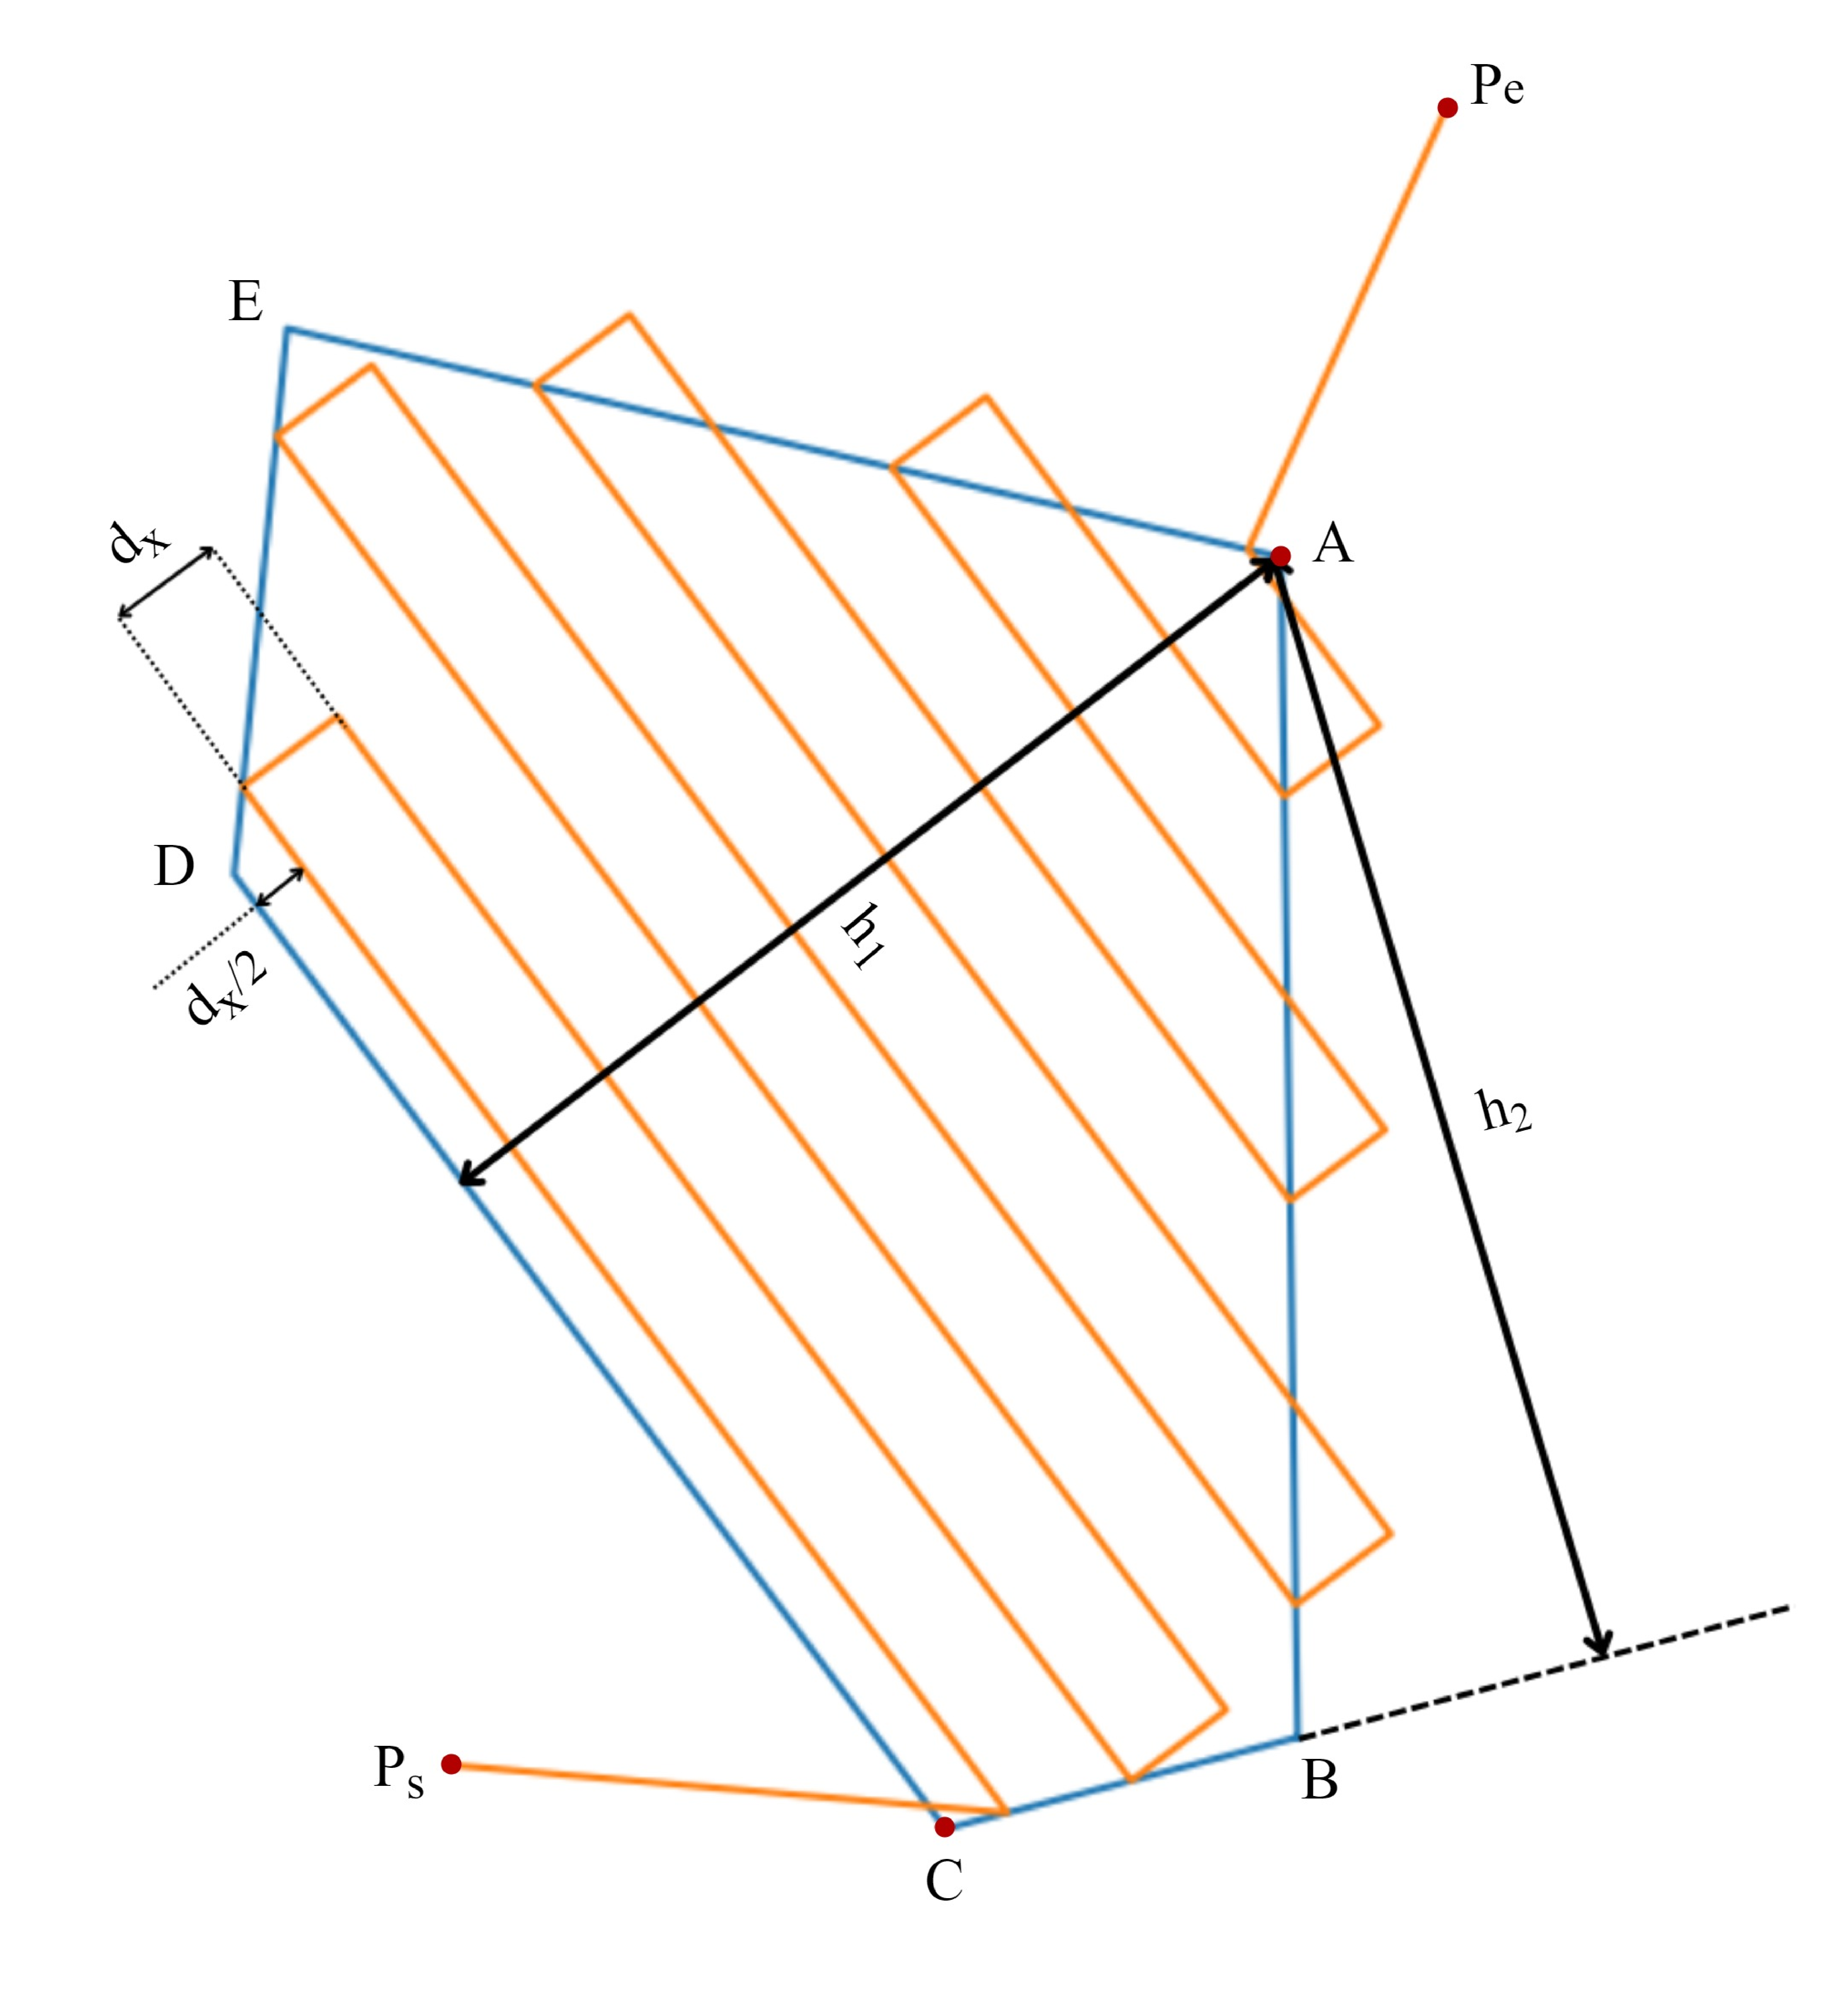
\includegraphics[width=0.5\textwidth]{chapter4/image/sweepline.drawio.pdf}
        \caption{Đường đi tiến lui được tạo bởi thuật toán RCPP}
        \label{fig:SW1}
    \end{figure}
    
Đường đi của robot quét qua khu vực khảo sát được gọi là đường bao phủ. Nó cần được thiết kế để tối đa hóa vùng phủ sóng và giảm thiểu thời gian bay. Trong điều khiển đội hình, không có sự phân tách khu vực khảo sát nào là cách tiếp cận thích hợp để giải quyết vấn đề này \cite{cabreira2019survey}. Bằng cách đi theo đường gấp khúc \cite{maza2007multiple} cho phép tạo ra các đường quét song song trong khu vực khảo sát. Vì vậy, để thỏa mãn các yêu cầu đã nêu, các đường quét cần đáp ứng các điều kiện sau: quét toàn bộ khu vực khảo sát; giảm thiểu sự chồng chéo giữa vùng phủ sóng của các đường quét; và tối ưu hóa số lượt rẽ của bầy Robot.

Trong đồ án này, các đường tiến lui (back and forth path) trong khu vực khảo sát được tạo ra bằng cách sử dụng kỹ thuật lập kế hoạch đường đi bao phủ \textbf{RCPP} (rotating calipers path planner) được đề xuất trong \cite{vasquez2020coverage}, và từ đó làm nó trơn tru hơn với nội suy đa thức spline.

\chapter{Experiments}
\section{Experimental Setup and Datasets}
\section{Results and Analysis}
This section presents the results of the experiments conducted to evaluate the performance of the sequential encounter encoding and the direct encoding in solving the optimization problem.
Because the number of variables and clauses in the CNF encoding when using standard method is too large, we benchmarked the performance of the two encoding methods on a smaller generated dataset.

\subsection{Comparison of Sequential Encounter Encoding and Standard Encoding}

The dataset was generated using the \texttt{input/generate.py} script, which is included in the source code repository.
It is stored in the \texttt{input} directory in the repository.
The dataset used in the experiments was generated using the following parameters:
\begin{itemize}
    \item Number of items: 8
    \item Number of transactions: 28
\end{itemize}

After generating the dataset, the optimization problem was encoded into CNF format using the sequential encounter encoding and the standard encoding.
With timeout 900ms and 1GB memory limit, we ran the Kissat SAT Solver on the CNF file to find all solutions.
The number of clauses and variables in the CNF encoding for each encoding method is shown in Figure \ref{fig:4_1} when Minimum Support is increased from 0.1 to 0.9 (10\% to 90\% of the total transactions).

% figure
\begin{figure}[H]
    \centering
    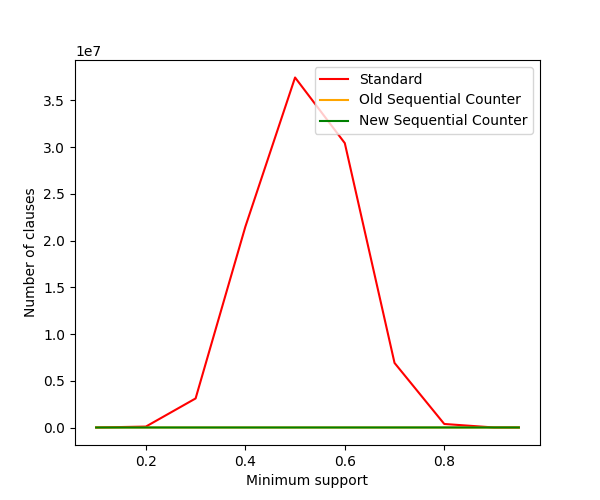
\includegraphics[width=1\textwidth]{chapter4/image/n_trans_28_clauses.png}
    \caption{Comparison of the number of clauses in the CNF encoding of the optimization problem using the sequential encounter encoding and the standard encoding.}
    \label{fig:4_1}
\end{figure}

This graph illustrates a notable difference between the number of clauses in the CNF encoding
utilizing the sequential encounter encoding compared to the standard encoding method. Particularly, it demonstrates that the sequential encounter encoding results in a significantly smaller number of clauses and variables.

Of special interest is the observation that the number of clauses generated by the standard encoding reaches a peak value,
approximately 35 million clauses, as the minimum support approaches the midpoint threshold.
This suggests a critical point where the standard encoding method generates an overwhelming number of clauses,
highlighting the potential inefficiency and scalability issues associated with this approach.

Additionally, the number of clauses generated by the sequential encounter encoding method appears to remain consistently low,
maintaining stability across various levels of minimum support.
This suggests that the sequential encounter encoding method is capable of producing fewer clauses while still ensuring the efficiency of the encoding process,
thus keeping the data analysis process manageable even as the constraints grow larger.

In addition to comparing the number of clauses, we also compared the time taken to find all solutions using both methods.
The results are shown in Figure \ref{fig:4_2}.
% figure
\begin{figure}[H]
    \centering
    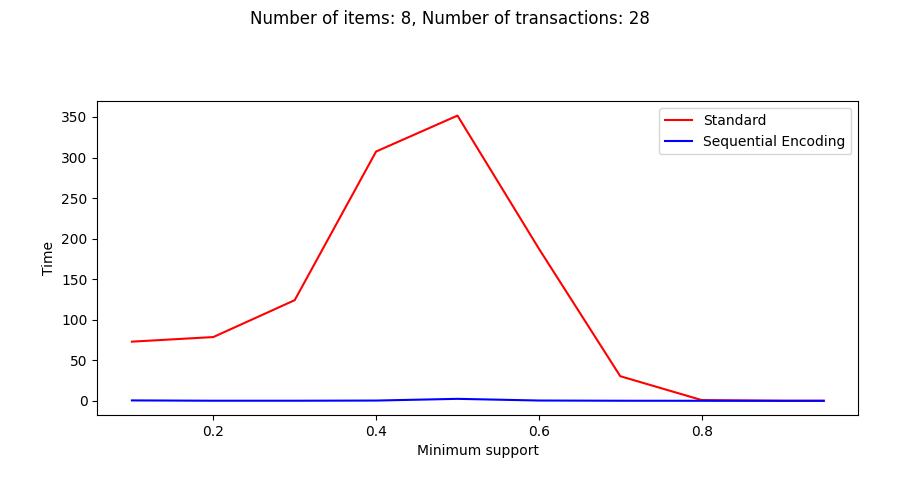
\includegraphics[width=1\textwidth]{chapter4/image/n_trans_28_time.png}
    \caption{Comparison of the time taken to find all solutions using the sequential encounter encoding and the standard encoding}
    \label{fig:4_2}
\end{figure}

The graph indicates that the sequential encounter encoding method consistently outperforms the standard encoding method in terms of time efficiency.
Even as the complexity of the problem increases, the sequential encounter encoding method demonstrates faster solution-finding times,
highlighting its superiority not only in minimizing the number of clauses but also in accelerating the solution discovery process.

However, it's worth noting that while the number of variables may increase, this increment is negligible compared to the significant reduction in the number of clauses.
\begin{figure}[H]
    \centering
    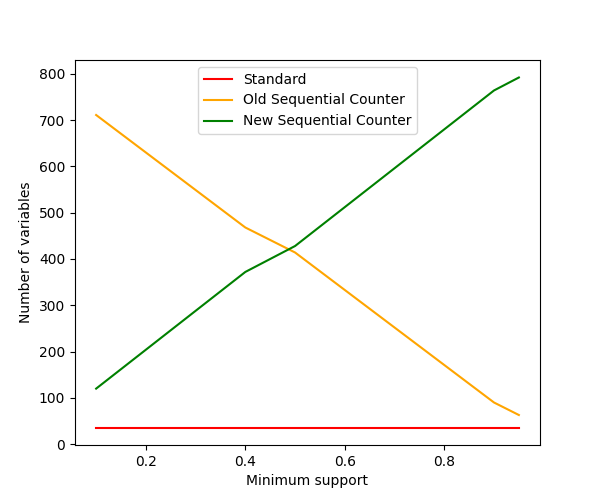
\includegraphics[width=1\textwidth]{chapter4/image/n_trans_28_vars.png}
    \caption{Comparison of the number of variables in the CNF encoding of the optimization problem using the sequential encounter encoding and the standard encoding.}
    \label{fig:4_3}
\end{figure}

This observation underscores the efficiency of the sequential encounter encoding method in striking a balance between the complexity of the problem and the computational resources required.
Despite the slight increase in variables, the overall computational overhead remains substantially lower,
making the sequential encounter encoding method a promising approach for tackling large-scale constraint satisfaction problems.

In addition, the experiments were conducted using various combinations of parameters to evaluate the performance of the sequential encounter encoding and the standard encoding in solving the optimization problem. By varying the number of transactions from 26 to 28 and the minimum support from 0.1 to 0.9, we aimed to assess the scalability and efficiency of both encoding methods across different problem sizes and constraints.
\begin{itemize}
    \item Number of items: 8
    \item Number of transactions: 26 to 28
    \item Minimum Support: 0.1 to 0.9
\end{itemize}

Table \ref{tab:4_1} presents the results obtained from these experiments.
It provides a comprehensive comparison of the number of variables, clauses, solutions, and time taken for each combination of parameters using both the standard encoding and the sequential encounter encoding.
\begin{table}[H]
    \centering
    \caption{Comparison of the number of variables, clauses, solutions, and time taken to find all solutions using the sequential encounter encoding and the standard encoding}
    \label{tab:4_1}
    \begin{tabular}{|c|c|r|r|r|r|r|r|r|r|}
        \hline
        \multirow{2}{*}{\textbf{Trans}} & \multirow{2}{*}{\textbf{Min Supp}} & \multicolumn{4}{r|}{\textbf{Standard Encoding}} & \multicolumn{4}{r|}{\textbf{Sequential Encounter}}                                                                                                    \\ \cline{3-10}
                                        &                                    & \textbf{Vars}                                   & \textbf{Clauses}                                   & \textbf{Sols} & \textbf{Time} & \textbf{Vars} & \textbf{Clauses} & \textbf{Sols} & \textbf{Time} \\ \hline
        26                              & 0.20                               & 34                                              & 65,935                                             & 27            & 21.03         & 190           & \textbf{ 774}    & 27            & \textbf{0.11} \\ \hline
        26                              & 0.30                               & 34                                              & 657,955                                            & 17            & 31.15         & 242           & \textbf{ 987}    & 17            & \textbf{0.10} \\ \hline
        26                              & 0.40                               & 34                                              & 5,311,890                                          & 7             & 67.28         & 320           & \textbf{1,314}   & 7             & \textbf{0.08} \\ \hline
        26                              & 0.50                               & 34                                              & 9,657,855                                          & 6             & 87.12         & 372           & \textbf{1,537}   & 6             & \textbf{0.13} \\ \hline
        26                              & 0.60                               & 34                                              & 7,726,315                                          & 2             & 40.67         & 450           & \textbf{1,879}   & 2             & \textbf{0.09} \\ \hline
        26                              & 0.70                               & 34                                              & 1,562,430                                          & 1             & 4.92          & 528           & \textbf{2,230}   & 1             & \textbf{0.02} \\ \hline
        26                              & 0.80                               & 34                                              & 230,385                                            & 1             & 0.57          & 580           & \textbf{2,469}   & 1             & \textbf{0.01} \\ \hline
        26                              & 0.90                               & 34                                              & 2,755                                              & 1             & 0.01          & 658           & 2,835            & 1             & 0.01          \\ \hline
        26                              & 0.95                               & 34                                              & 480                                                & 1             & 0.00          & 684           & \textbf{2,959}   & 1             & \textbf{0.01} \\ \hline
        27                              & 0.10                               & 35                                              & 499                                                & 89            & 37.55         & 116           & \textbf{ 467}    & 89            & \textbf{0.68} \\ \hline
        27                              & 0.20                               & 35                                              & 80,878                                             & 35            & 39.81         & 197           & \textbf{ 791}    & 35            & \textbf{0.13} \\ \hline
        27                              & 0.30                               & 35                                              & 2,220,223                                          & 18            & 80.47         & 278           & \textbf{1,124}   & 18            & \textbf{0.11} \\ \hline
        27                              & 0.40                               & 35                                              & 8,436,433                                          & 8             & 124.90        & 332           & \textbf{1,351}   & 8             & \textbf{0.13} \\ \hline
        27                              & 0.50                               & 35                                              & 20,058,448                                         & 7             & 187.88        & 413           & \textbf{1,699}   & 7             & \textbf{0.24} \\ \hline
        27                              & 0.60                               & 35                                              & 13,038,043                                         & 3             & 72.68         & 494           & \textbf{2,056}   & 3             & \textbf{0.14} \\ \hline
        27                              & 0.70                               & 35                                              & 4,686,973                                          & 1             & 19.21         & 548           & \textbf{2,299}   & 1             & \textbf{0.05} \\ \hline
        27                              & 0.80                               & 35                                              & 296,158                                            & 1             & 1.43          & 629           & \textbf{2,671}   & 1             & \textbf{0.01} \\ \hline
        27                              & 0.90                               & 35                                              & 3,073                                              & 1             & 0.01          & 710           & \textbf{3,052}   & 1             & \textbf{0.01} \\ \hline
        27                              & 0.95                               & 35                                              & 499                                                & 1             & 0.00          & 737           & 3,181            & 1             & 0.01          \\ \hline
        28                              & 0.10                               & 36                                              & 547                                                & 58            & 72.94         & 120           & \textbf{ 500}    & 58            & \textbf{0.49} \\ \hline
        28                              & 0.20                               & 36                                              & 98,449                                             & 29            & 78.61         & 204           & \textbf{ 836}    & 29            & \textbf{0.08} \\ \hline
        28                              & 0.30                               & 36                                              & 3,108,274                                          & 13            & 124.10        & 288           & \textbf{1,181}   & 13            & \textbf{0.09} \\ \hline
        28                              & 0.40                               & 36                                              & 21,474,349                                         & 9             & 307.41        & 372           & \textbf{1,535}   & 9             & \textbf{0.30} \\ \hline
        28                              & 0.50                               & 36                                              & 37,442,329                                         & 6             & 351.73        & 428           & \textbf{1,776}   & 6             & \textbf{2.41} \\ \hline
        28                              & 0.60                               & 36                                              & 30,421,924                                         & 3             & 187.64        & 512           & \textbf{2,145}   & 3             & \textbf{0.34} \\ \hline
        28                              & 0.70                               & 36                                              & 6,907,069                                          & 1             & 30.33         & 596           & \textbf{2,523}   & 1             & \textbf{0.07} \\ \hline
        28                              & 0.80                               & 36                                              & 376,909                                            & 1             & 0.91          & 680           & \textbf{2,910}   & 1             & \textbf{0.01} \\ \hline
        28                              & 0.90                               & 36                                              & 3,445                                              & 1             & 0.01          & 764           & \textbf{3,306}   & 1             & \textbf{0.01} \\ \hline
        28                              & 0.95                               & 36                                              & 547                                                & 1             & 0.00          & 792           & 3,440            & 1             & 0.01          \\ \hline
    \end{tabular}
\end{table}

From the table \ref{tab:4_1}, we can observe that as the minimum support increases,
the number of clauses and variables in the CNF encoding generally tends to increase for both encoding methods.
However, the sequential encounter encoding consistently generates a significantly smaller number of clauses and variables compared to the standard encoding.
This reduction in the size of the CNF encoding demonstrates the efficiency and effectiveness of the sequential encounter encoding method in representing the optimization problem.

Furthermore, the table also shows the time taken to find all solutions using each encoding method.
It is evident that the sequential encounter encoding outperforms the standard encoding in terms of time efficiency.
Even as the complexity of the problem increases with higher minimum support values, the sequential encounter encoding method demonstrates faster solution-finding times.
This highlights the advantage of using the sequential encounter encoding method for solving large-scale constraint satisfaction problems.

Overall, the experimental results support the superiority of the sequential encounter encoding method over the standard encoding method in terms of both the size of the CNF encoding and the time efficiency of finding solutions. These findings validate the effectiveness and scalability of the sequential encounter encoding approach in solving optimization problems with varying problem sizes and constraints.


\subsection{Sequential Encounter Encoding on Real-World Dataset}

We delve into the empirical evaluation of the sequential encounter encoding technique within the domain of frequent itemset mining. To ascertain the effectiveness and efficiency of this method, a series of comprehensive experiments were conducted using authentic datasets procured from the Frequent Itemset Mining Implementations (FIMI) and Constraint Programming for Itemset Mining (CP4IM) repositories.

The initial step involved an extensive preprocessing phase,
wherein the datasets were meticulously formatted to ensure compatibility with
the encoding algorithms. Subsequent to this preprocessing,
the datasets were encoded using only the sequential encounter encoding because the standard encoding method is not feasible due to the large number of variables and clauses generated.

The datasets selected for the experimental study are succinctly summarized
in Table \ref{tab:result_benchmark_real_datasets}.
The table provides an insightful juxtaposition of key metrics such as the number of variables,
clauses, and the computational time expended for each dataset.

\begin{table}[H]
    \centering
    \caption{Comparison of the number of variables, clauses, solutions, and time taken using the sequential encounter encoding and the standard encoding}
    \label{tab:result_benchmark_real_datasets}
    \begin{tabular}{|l|c|c|c|r|r|r|}
        \hline
        \multirow{2}{*}{\textbf{Dataset}} & \multirow{2}{*}{\textbf{Items}} & \multirow{2}{*}{\textbf{Trans}} & \multirow{2}{*}{\textbf{Min Supp}} & \multicolumn{3}{r|}{\textbf{Standard Encoding}}                                    \\ \cline{5-7}
                                          &                                 &                                 &                                    & \textbf{Vars}                                   & \textbf{Clauses} & \textbf{Time} \\ \hline
        zoo-1                             & 36                              & 101                             & 0.10                               & 1,245                                           & 5,489            & 0.06          \\
        primary-tumor                     & 31                              & 336                             & 0.10                               & 11,790                                          & 50,304           & 0.10          \\
        vote                              & 48                              & 435                             & 0.10                               & 19,614                                          & 81,411           & 0.17          \\
        soybean                           & 50                              & 630                             & 0.10                               & 40,360                                          & 165,745          & 0.36          \\
        chess                             & 75                              & 3,196                           & 0.10                               & 1,025,990                                       & 4,212,750        & 9.45          \\
        chess                             & 75                              & 3,196                           & 0.20                               & 2,048,710                                       & 8,455,790        & 18.16         \\
        chess                             & 75                              & 3,196                           & 0.30                               & 3,068,234                                       & 12,787,491       & 43.26         \\
        chess                             & 75                              & 3,196                           & 0.40                               & 4,090,954                                       & 17,235,011       & 38.59         \\
        chess                             & 75                              & 3,196                           & 0.50                               & 5,110,478                                       & 21,770,553       & 52.63         \\
        mushroom                          & 119                             & 8,124                           & 0.10                               & 6,613,018                                       & 26,853,806       & 65.64         \\
        mushroom                          & 119                             & 8,124                           & 0.20                               & 13,209,706                                      & 54,226,732       & 187.69        \\
        mushroom                          & 119                             & 8,124                           & 0.30                               & 19,814,518                                      & 82,293,931       & 798.24        \\ \hline
    \end{tabular}
\end{table}

Observing Table \ref{tab:result_benchmark_real_datasets}, it becomes evident
that the sequential encounter encoding method demonstrates varied performance benefits across different datasets.
For instance, the 'zoo-1' dataset, characterized by 36 items and 101 transactions,
was encoded with significantly fewer variables and clauses, resulting in an impressively swift computation time of
only 0.06 seconds. This marked efficiency showcases the potential of the sequential encounter encoding in dealing with
smaller datasets.

Conversely, as we scrutinize datasets with a larger number of transactions and items,
such as 'chess' and 'mushroom', we notice a discernible trend of increased complexity.
The 'chess' dataset at a 0.10 minimum support level demanded over a million variables in the standard encoding approach,
with a consequent computational time of approximately 9.45 seconds.
The escalation in complexity is palpable when the minimum support is altered,
impacting the number of solutions and, inevitably, the time required for computation.

The 'mushroom' dataset further elucidates the scalability challenges,
where the number of variables peaks for the standard encoding at a 0.30 minimum support,
with an accompanying computational time that extends to a substantial 798.24 seconds.
This starkly contrasts with the lesser demanding 'zoo-1' and 'primary-tumor' datasets,
underscoring the necessity of an encoding method that can adeptly adapt to varying dataset sizes and complexities.

The table emphatically highlights the nuanced relationship between dataset characteristics and
encoding performance. The sequential encounter encoding method's capability to
effectively manage the number of variables and clauses without compromising
on the discovery of solutions is a testament to its robustness.
Additionally, the encoding method's impact on computational time is of paramount importance,
as it directly correlates with the practicality of the approach in real-world applications.

In summary, the experimental evaluation substantiates the hypothesis that sequential encounter encoding can be a potent alternative to standard encoding in itemset mining,
particularly when tailored to the dataset at hand. These findings advocate for a discerning application of encoding techniques in itemset mining, with the sequential encounter
encoding method emerging as a significant contender in the field.

\chapter{Conclusions}
\section{Conclusion}

In conclusion, this study has provided a comprehensive exploration of itemset mining tasks and introduced innovative techniques for optimizing the encoding process. We began by elucidating the fundamentals of itemset mining, highlighting its significance in various domains such as retail, healthcare, and bioinformatics. The encoding of itemset mining problems into SAT instances was meticulously examined, showcasing the sequential encounter encoding approach as a promising alternative to traditional methods. By leveraging the sequential nature of transactional data, sequential encounter encoding offers a more efficient and scalable solution for itemset mining tasks.

Furthermore, we delved into the application of the standard method $C_{n-k+1}$
for encoding itemset mining constraints, shedding light on its limitations and challenges, particularly in handling large datasets. Through a comparative analysis, we demonstrated the advantages of sequential encounter encoding in reducing computational complexity and improving mining efficiency.

Moving forward, there are several avenues for future research. Expanding the application of sequential encounter encoding to different problem domains and refining the encoding process to accommodate diverse datasets are promising areas for exploration. Additionally, investigating hybrid approaches that combine sequential encounter encoding with other optimization techniques could yield further improvements in mining performance.

Overall, this study contributes to the advancement of itemset mining methodologies and lays the groundwork for future research endeavors aimed at enhancing the efficiency and effectiveness of mining algorithms. By embracing innovative approaches such as sequential encounter encoding, we can unlock new insights from large-scale datasets and drive progress in data mining and analytics.
\section{Thí nghiệm với mô hình robot là các chất điểm trong không gian 3D}
\label{sec:result}
Phần này trình bày các thí nghiệm mô phỏng đội hình máy bay không người lái UAV (Unmanned Aerial Vehicle) thực hiện chiến lược bao phủ để tuần tra, giám sát một khu vực yêu cầu có dạng đa giác lồi. Trình mô phỏng được thiết kế trên Python sử dụng thư viện MatplotlibV trong đó mỗi UAV được mô hình như một chất điểm. Kết quả này đã được công bố trong bài báo tại Hội nghị quốc tế lần từ 11 về điều khiển, tự động hóa và khoa học thông tin ICCAIS tổ chức tháng 11/2022 tại Hà Nội.

Trong các thí nghiệm mô phỏng, Robot được mô phỏng dưới dạng các hạt với các tham số của FOV là $\alpha = 0.15rad$, $\beta = 0.22 rad$, $\%overlapping$ $x = 30\%$ và phạm vi cảm nhận của nó là giống như đĩa tròn với khả năng phát hiện chướng ngại vật khi tiếp xúc. Độ cao bay và vận tốc tối đa của Robot lần lượt được đặt ở mức $20m$ và $10m/s$ . Các thông số điều khiển hành vi đã được đặt là $a_{m2g} = a_{kf} = 3.3, b_{m2g} = b_ {kf} = 1, a_ {Ath} = 3.0, b_ {Ath} = 4.0, a_ {adr} = 1,5, b_ {adr} = 2,4$. 

$h = 20m$

$|v|<10$m/s

\begin{figure}
\centering
    %\hspace{-0.5cm}
    \begin{subfigure}[b]{0.8\textwidth}
    \centering
    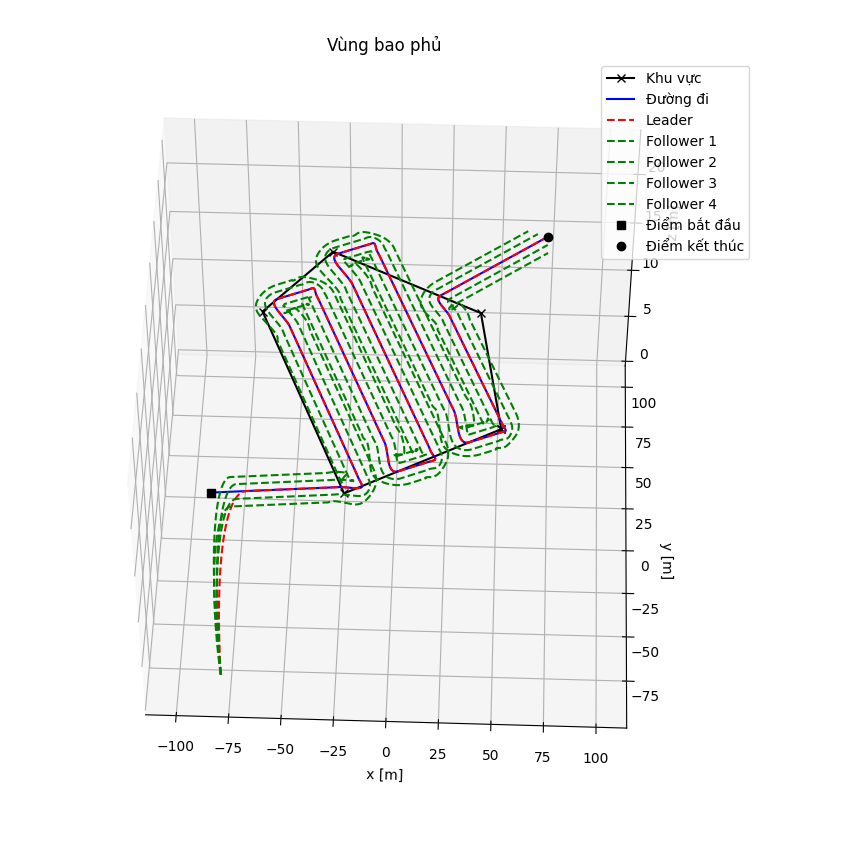
\includegraphics[width=\textwidth]{chapter5/image/coverage1.png}
    \caption{}
    \label{fig:1}
    \end{subfigure}
    %\hspace{-0.5cm}
    \begin{subfigure}[b]{0.8\textwidth}
    \centering
    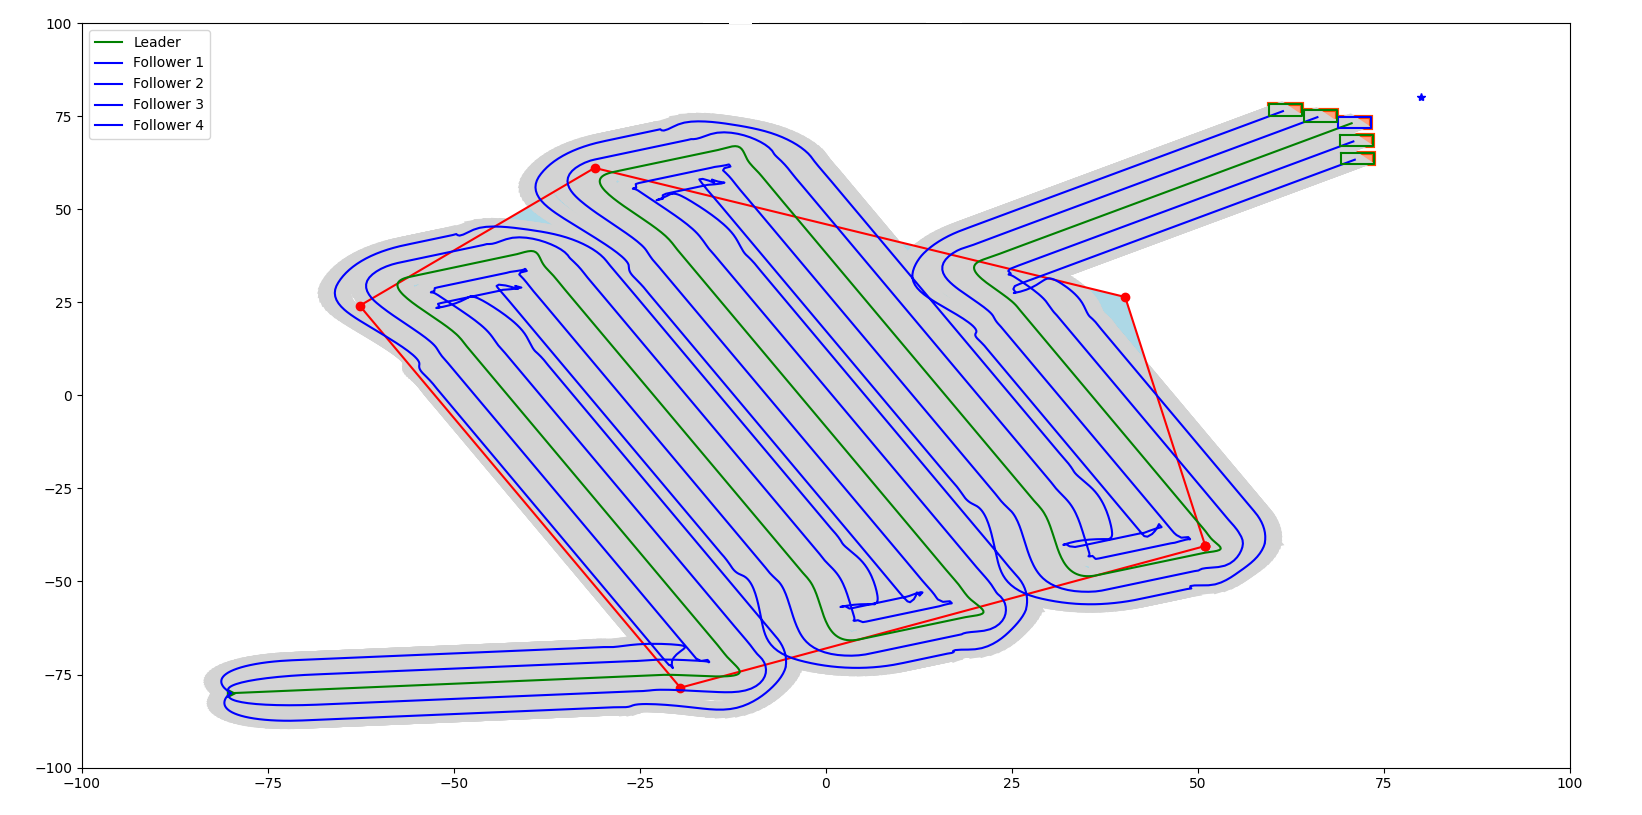
\includegraphics[width=\textwidth]{chapter5/image/coverage.png}
    \caption{}
    \label{fig:2}
    \end{subfigure}
    \caption{Phạm vi bao phủ đội hình chữ V}
    \label{fig:coverarea5Robot}
\end{figure}

\begin{figure}
\centering
    %\hspace{-0.5cm}
    \begin{subfigure}[b]{0.8\textwidth}
    \centering
    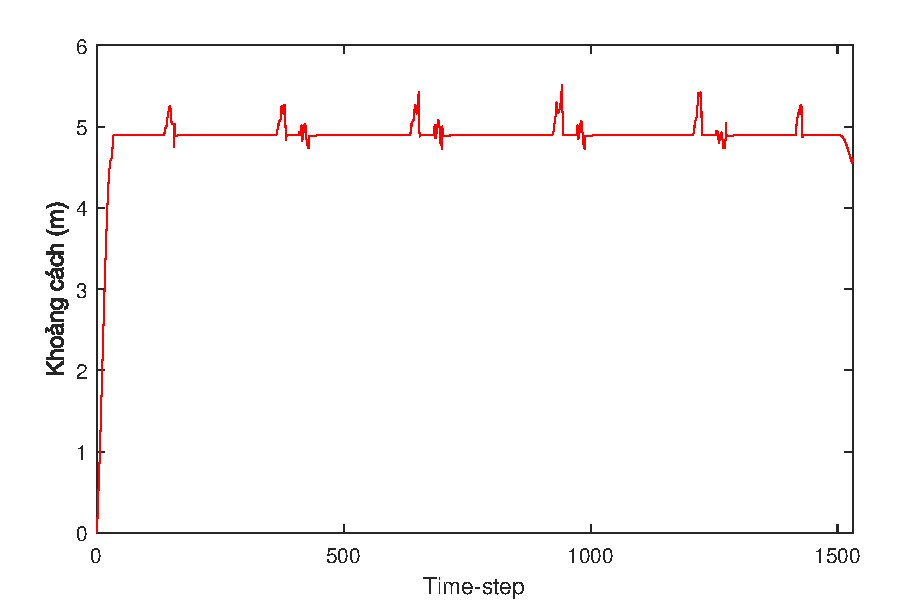
\includegraphics[width=\textwidth]{chapter5/image/Median_Dis.pdf}
    \caption{Khoảng cách trung vị giữa 2 robot liên tiếp}
    \label{fig:Distance5Robot}
    \end{subfigure}
    %\hspace{-0.5cm}
    \begin{subfigure}[b]{0.8\textwidth}
    \centering
    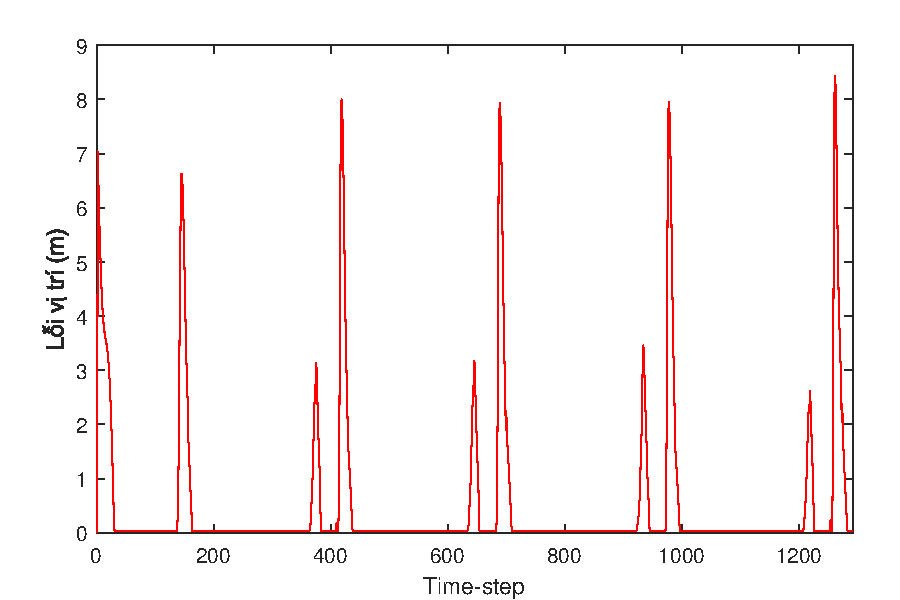
\includegraphics[width=\textwidth]{chapter5/image/Median_Err.pdf}
    \caption{Trung vị về sai số vị trí vị trí follower và các điểm virtual target}
    \label{fig:err5Robot}
    \end{subfigure}
    \caption{Kết quả sự ổn định của quá trình di chuyển đội hình chữ V}
    \label{fig:5Ro}
\end{figure}


Đầu tiên, đầu vào sẽ là khu vực cần được khảo sát có dạng hình polygon ngũ giác. Thuật toán sẽ tiến hành xây dựng và lập đường đi bao phủ cho Leader. Từ đó, quỹ đạo của Leader được hình thành. Trong quá trình di chuyển, Leader sẽ tạo ra cấu trúc ảo có dạng hình chữ V để các Followers có thể di chuyển và bám theo quỹ đạo . Phần này sẽ tiến hành thực hiện một thử nghiệm mô phỏng thể hiện thông qua Hình.\ref{fig:coverarea5Robot}. Trong đó, các đường màu đen là vùng giới hạn của khu vực quan tâm, đường màu đỏ là quãng đường được xây dựng dành riêng cho Leader. Các đường màu xanh lá cây thể hiện được quỹ đạo của 4 robot Followers bám theo để tạo thành cấu trúc hình chữ V \footnote{Đội hình chữ V với 5 Robots \url{https://youtu.be/A5u8xT-GqYQ}}


Kết quả mô phỏng trong Hình.\ref{fig:coverarea5Robot} cho thấy bầy Robot duy trì đội hình chữ V và quét qua toàn bộ vùng khảo sát với tỉ lệ cao là $98.69\%$. Ngoài ra, Hình.\ref{fig:Distance5Robot} chỉ ra rằng mức độ ổn định của đội hình robot trong quá trình di chuyển. Qua đó thấy rằng khi đội hình di chuyển trên đoạn đường thẳng, giá trị trung vị khoảng cách tương đối giữa hai robot liên tiếp luôn được duy trì ở mức ổn định so với tham số đội hình yêu cầu $\ell=4.89 m$, sự giao động chỉ xuất hiện ở các khúc rẽ trong đường đi với độ lệch chuẩn là  $6.44\%$-$12.68\%$. Đối với lỗi vị trí trong Hình \ref{fig:err5Robot}, cũng như trung vị khoảng cách vị trí hiện tại của các followers với các điểm vị trí ảo do leader tạo ra, đường đi thẳng có giá trị trung vị của các vị trí lỗi từ $3.5 m$ đến $8.5m $  khi nó giao động mạnh ở các khúc rẽ của đường zig zac dẫn tới việc robot leader đổi hướng nhanh. Tuy nhiên, nhờ vào hành vi duy trì đội hình được chỉ ra trong chương 2, đội hình chữ V dần dần quay lại trạng thái ổn định. 


Tiếp theo, phần này thực hiện khảo sát thời gian khi bầy robot tiến hành quét qua các khu vực cụ thể. Quá trình mô phỏng sẽ tạo ra ngẫu nhiên 20 vùng khác nhau về diện tích và hình dạng được mô tả trong bảng \ref{tab:Scoverage1}.

\begin{table}[H]
\centering
\caption{Bảng mô tả kích thước các khu vực thử nghiệm}
\label{tab:Scoverage1}
\begin{tabular}{|l|c|c|c|c|c|c|c|}
\hline
\textbf{Map}      & \textit{1}  & \textit{2}  & \textit{3}  & \textit{4}  & \textit{5}  & \textit{6}  & \textit{7}  \\ \hline
\textbf{Area ($m^2$)} & 10789.23    & 8550.85     & 9260.03     & 7966.47     & 8088.73     & 5600.21     & 3408.49  \\ \hline
\textbf{Map}      & \textit{8}  &\textit{9}   & \textit{10} & \textit{11} & \textit{12} & \textit{13} & \textit{14}    \\ \hline
\textbf{Area ($m^2$)}  & 5706.51   & 10224.71    & 9964.78     &9742.46     & 7705.11     & 11979.95    & 24842.79 \\ \hline
\textbf{Map}     & \textit{15} & \textit{16} & \textit{17}   & \textit{18} & \textit{19} & \textit{20}  & - \\ \hline
\textbf{Area ($m^2$)} & 9805.33     & 14419.30  & 10455.92    & 10535.73    & 10846.23    & 14382.34  & - \\ \hline
\end{tabular}
\end{table}

Với 20 vùng bao phủ này, mỗi vùng sẽ được thử nghiệm với số lượng các con robot khác nhau với các mốc 3, 5, 7. Như trên hình \ref{fig:3r},\ref{fig:5r},\ref{fig:7r}:

\begin{figure}[H]
    \centering
    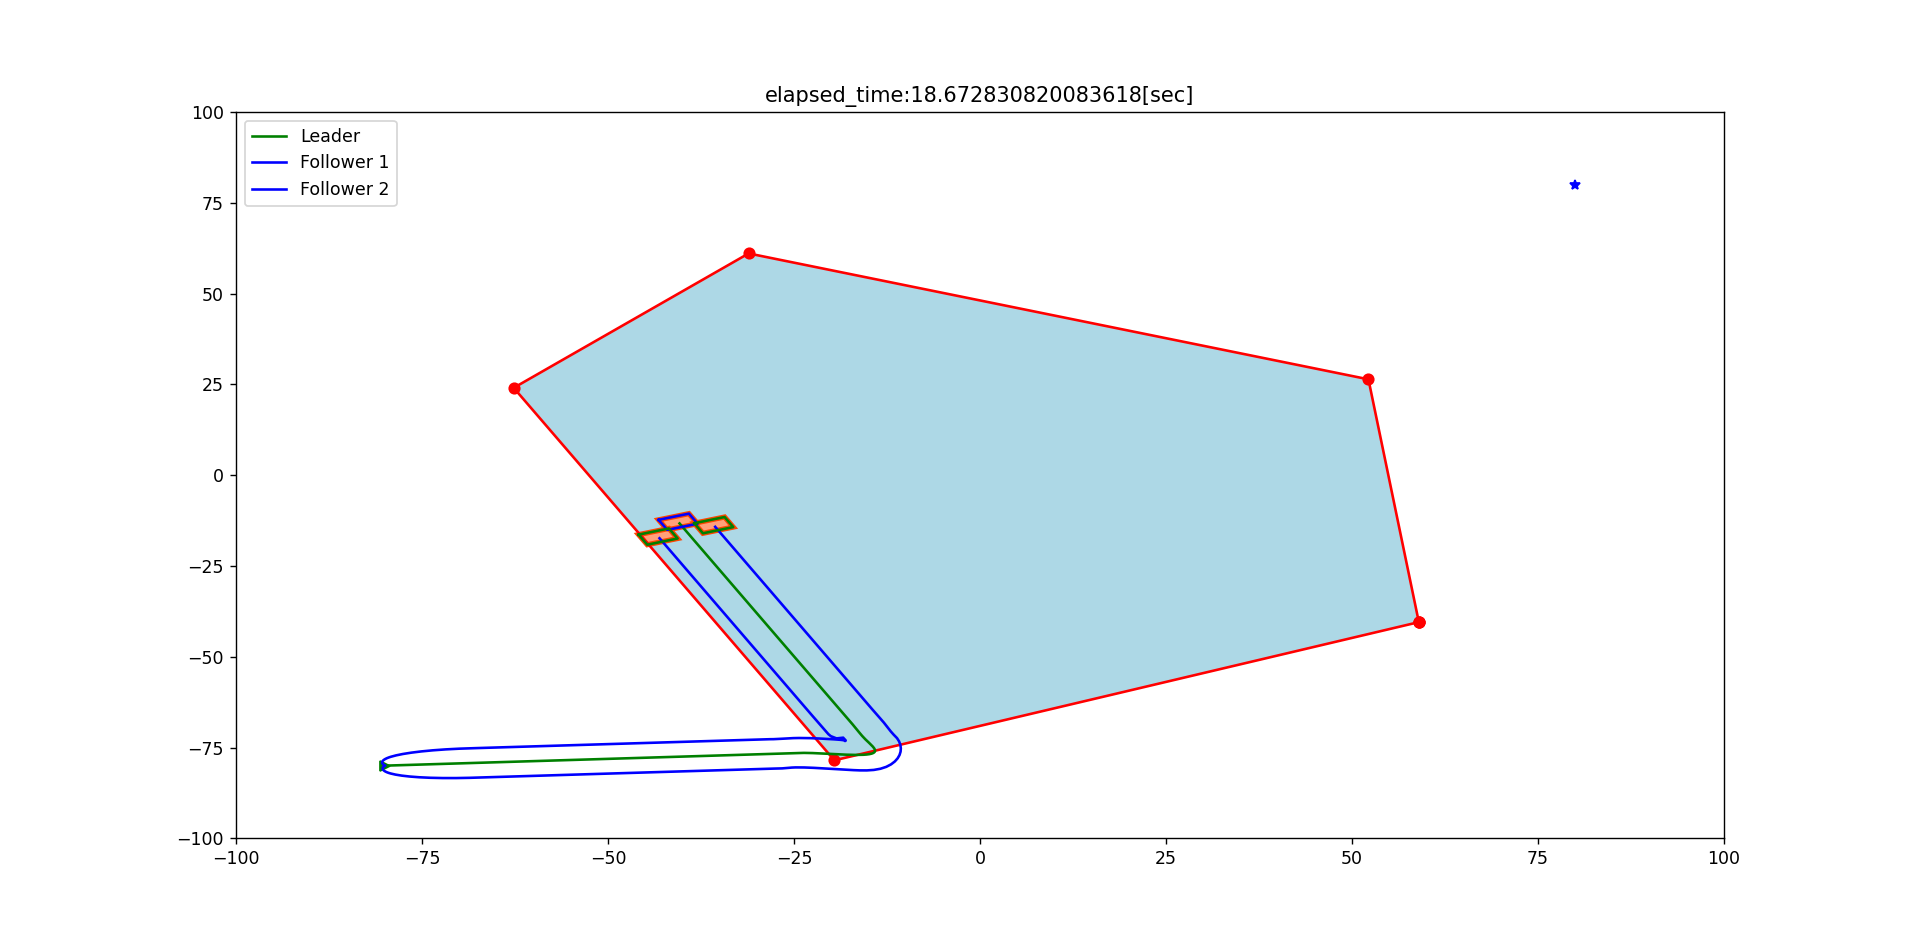
\includegraphics[width=0.8\textwidth]{chapter5/image/3robot.png}
    \caption{Mô phỏng quá trình 3 robot thực hiện quá trình bao phủ}
    \label{fig:3r}
\end{figure}

\begin{figure}[H]
    \centering
    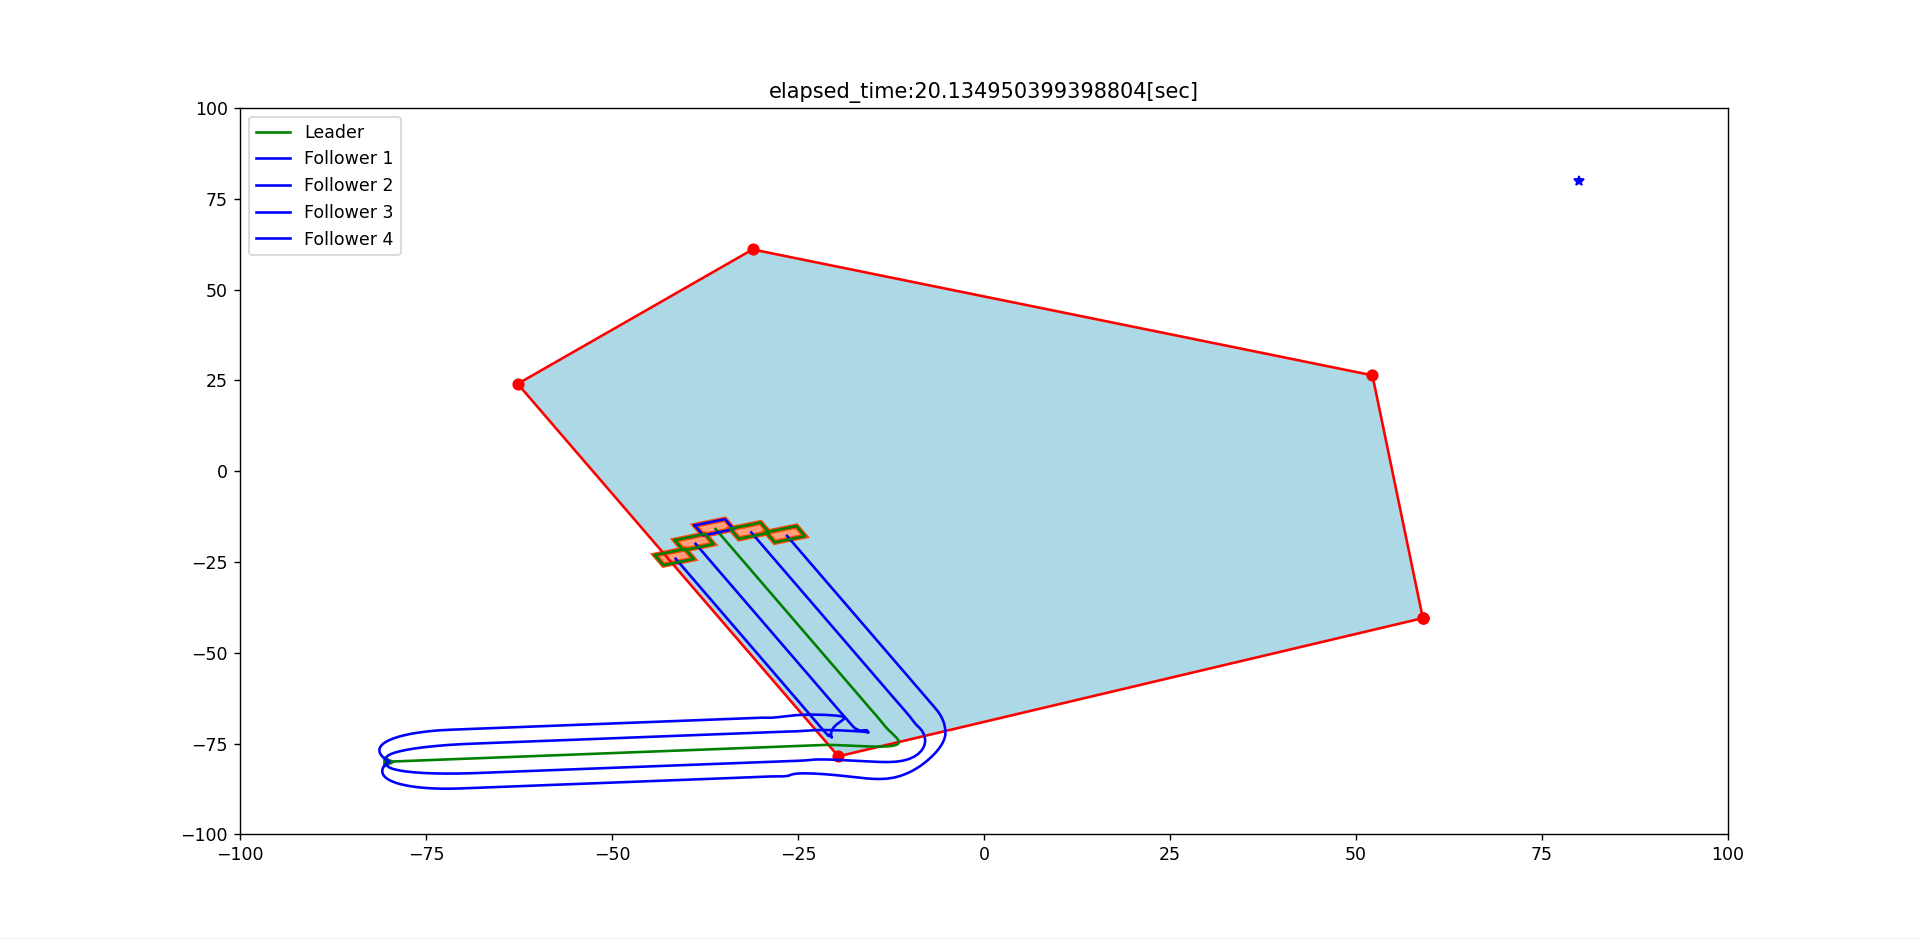
\includegraphics[width=0.8\textwidth]{chapter5/image/5robot.png}
    \caption{Mô phỏng quá trình 5 robot thực hiện quá trình bao phủ}
    \label{fig:5r}
\end{figure}

\begin{figure}[H]
    \centering
    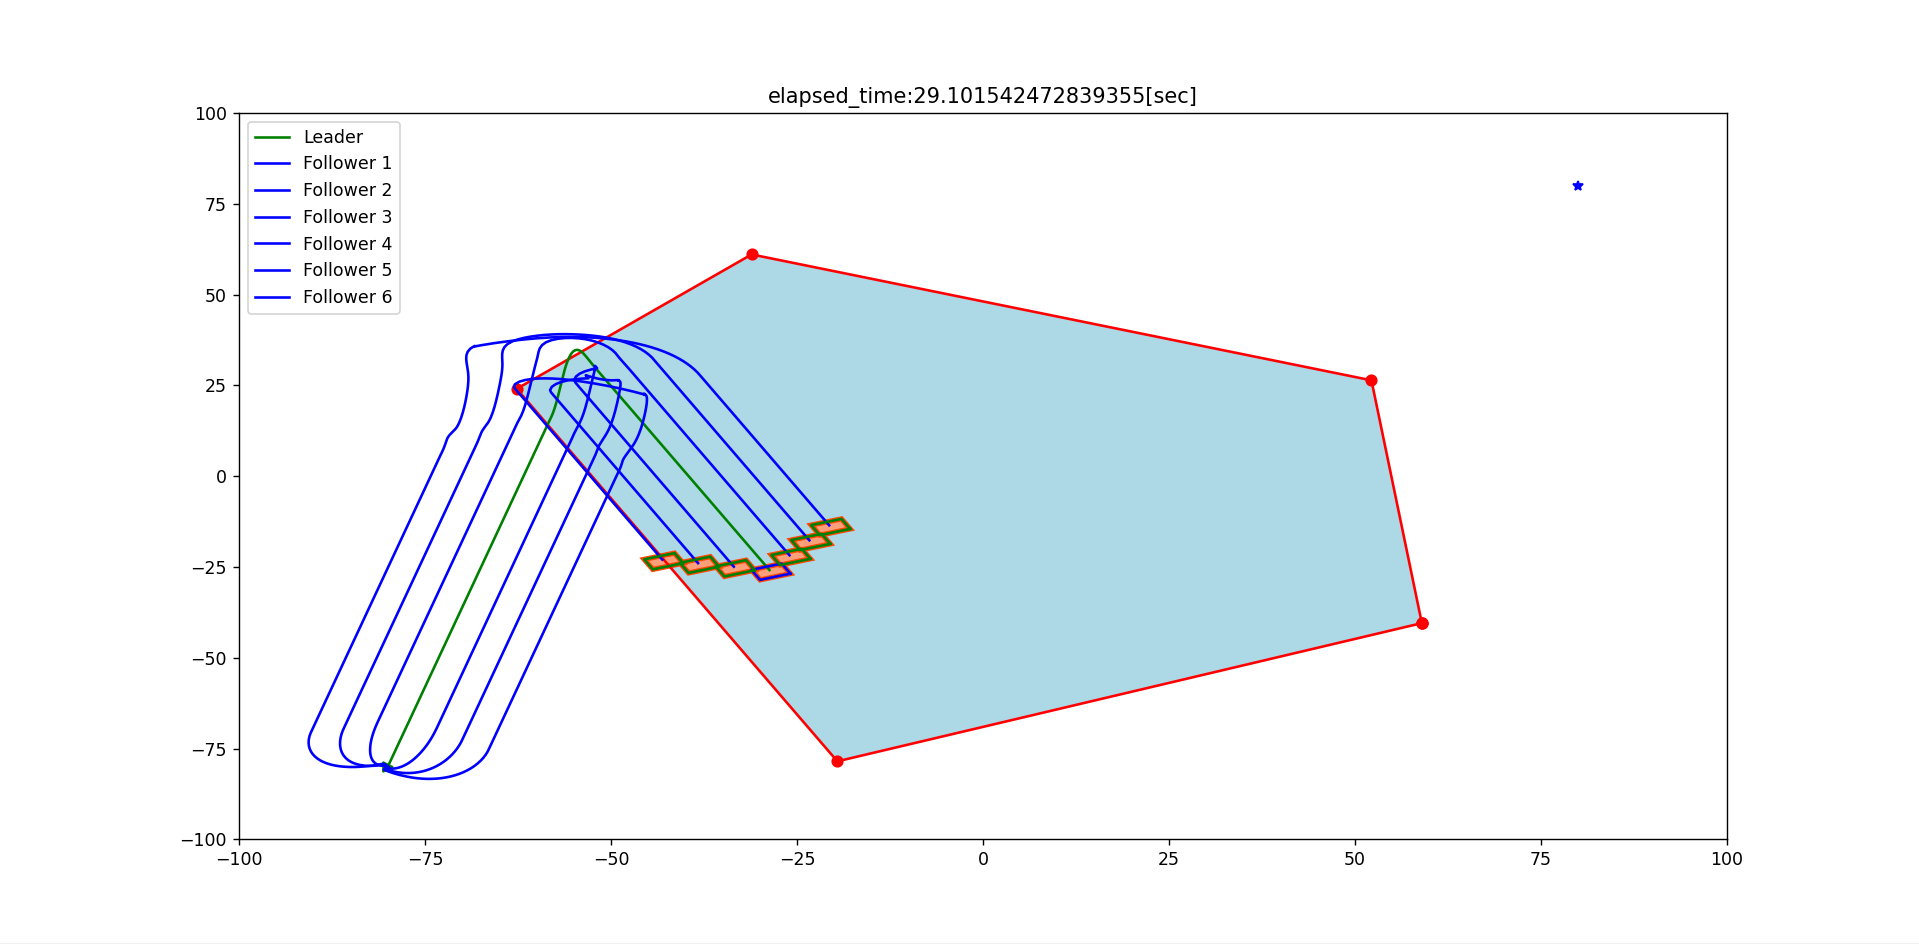
\includegraphics[width=0.8\textwidth]{chapter5/image/7robot.png}
    \caption{Mô phỏng quá trình 7 robot thực hiện quá trình bao phủ}
    \label{fig:7r}
\end{figure}

Cùng với đó, các robot sẽ được đưa vào thử nghiệm các trên 3 giải thuật khác nhau bao gồm: Đường đi bao phủ tốt nhất(Op-RCPP) được mô tả trong phần \ref{sec:Oppath}, đường đi bao phủ với nhiều khúc quay nhất(nonOp-RCPP)(đây là thuật toán tương tự như op-RCPP nhưng sẽ chọn số lượng đường rẽ tối đa thay vì chọn số lượng đường rẽ tối thiểu), và thuật toán lập đường đi bao phủ dựa trên chia lưới(grid-base coverage path planning) trong bài \cite{nam2016approach} với mục tiêu so sánh. Trong mỗi kịch bản, vị trí xuất phát ban đầu của Robot đều được giữ cố định tại điểm có toạ độ: PS = $(-80;-80;0)$, và vị trí kết thúc hành trình có toạ độ là : PE = $(80;80;0)$. Vì vậy sẽ có tổng cộng là 180 kịch bản được mô phỏng để lấy kết quả.

\begin{figure}[h!]
    \centering
    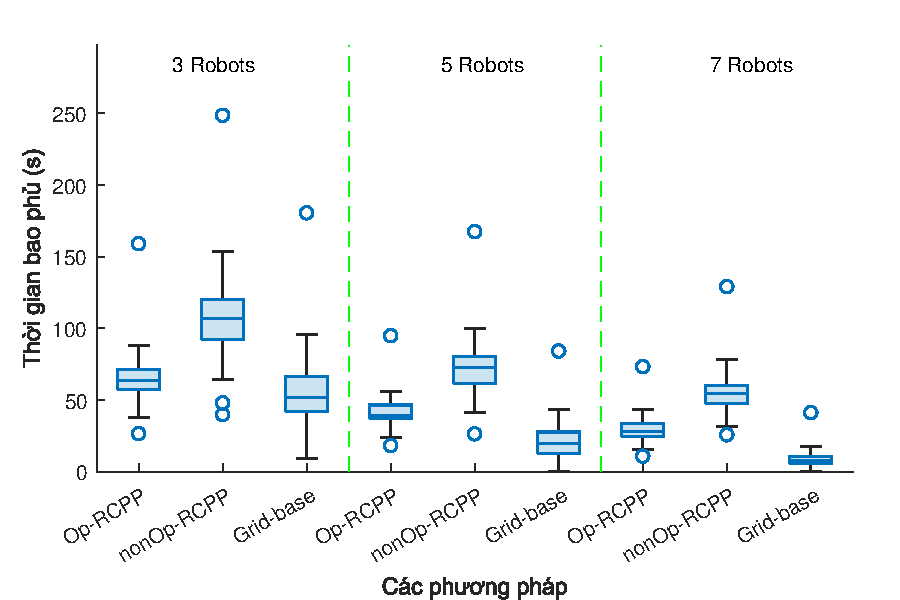
\includegraphics[width=0.8\textwidth]{chapter5/image/CoverageTime.pdf}
    \caption{Thời gian bao phủ với đội hình robot chữ V}
    \label{fig:cov}
\end{figure}

Dựa vào kết quả thu được hình \ref{fig:cov}, có thể thấy được rằng sử dụng thuật toán đường đi tối ưu (Op-RCPP) sẽ thu được kết quả tốt hơn về mặt thời gian bay cũng đồng nghĩa với việc giúp tối ưu về mặt năng lượng khi di chuyển mà vẫn đạt được mục đích bao phủ gần như tuyệt đối. Tuy nhiên khi so sánh với thuật toán không tối ưu(nonOp-RCPP), thuật toán tối ưu đường đi(Op-RCPP) thì sẽ mang lại khả năng di chuyển nhanh hơn gấp $1.8$ lần nhưng độ độ bao phủ lại ít hơn $0.3\% - 8\%$. Điều này xảy ra là bởi vì thuật toán không tối ưu sẽ lựa chọn hướng di chuyển có nhiều góc quay hơn nên sẽ có thể bao phủ tốt hơn tuy vậy thời gian cũng tăng lên đáng kể. 


Đối với thuật toán lập đường đi bao phủ dựa trên chia lưới(Grid-base), trước khi tiến hành khảo sát, do thuật toán còn phụ thuộc vào việc chia độ rộng của lưới hay là độ lớn của độ rộng sải cánh $dx$ của đội hình chữ V, nên sẽ để lộ ra các vùng viền bao quanh bản đồ không thể quét qua làm giảm độ bao phủ, độ bao phủ chỉ tập trung vào vùng trung tâm. Với kích thước của $dx$ càng lớn thì phần không được che phủ càng nhiều. Tuy nhiên thời gian di chuyển sẽ có thể nhanh hơn thuật toán tối ưu đường đi, mặc dù vậy thuật toán này lại có một yếu điểm là trong một số vùng diện tích quá nhỏ không đáp ứng đủ độ rộng sải cánh của đội hình bay dẫn đến trường hợp không thể chia được ô nên thuật toán không thể hoạt động dẫn việc không tạo được đường đi bao phủ. Như vậy thuật toán tối ưu đường đi mang lại kết quả khả quan nhất về mặt thời gian bay bao phủ chỉ phù hợp cho một con robot di chuyển, bao phủ.

 Ngoài ra, khi tăng số lượng robots trong đội hình, thời gian bay giảm. Đặc biệt là trong phương pháp tối ưu đường đi bao phủ, thời gian bay của đội hình chữ V với 5 hoặc 7 robots xấp xỉ giảm $38.84\%$ và $55.58\%$ so với việc đội hình có 3 robots. Nguyên nhân là do khi số lượng robots tăng, sự bao phủ của bầy robot tăng dẫn đến số đường đi giảm.

\begin{figure}[H]
    \centering
    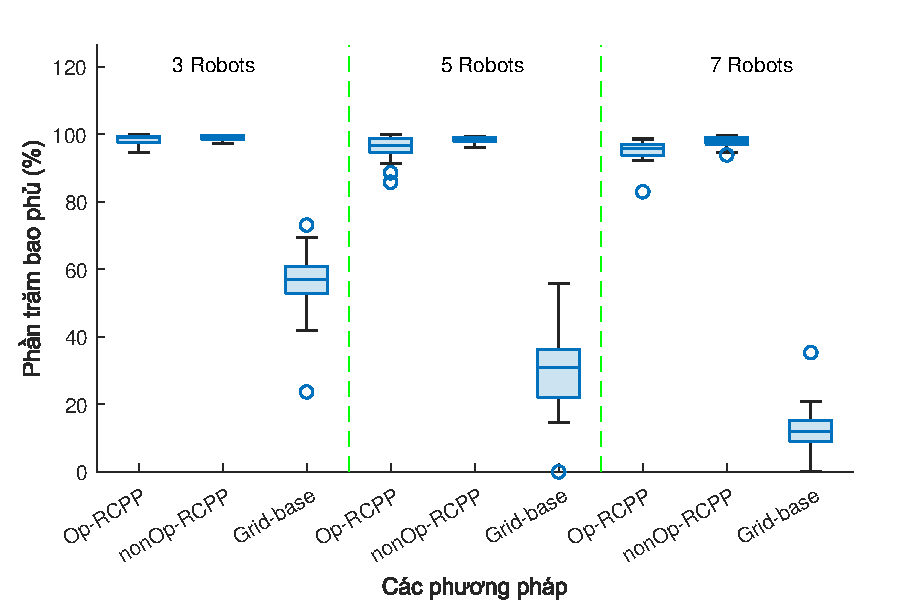
\includegraphics[width=0.8\textwidth]{chapter5/image/CoveragePer.pdf}
    \caption{Tỷ lệ bao phủ với đội hình robot chữ V}
    \label{fig:covPer}
\end{figure}

Kết quả thu được trong Hình.\ref{fig:covPer} cho thấy tỉ lệ che phủ của đội hình Robot chữ V với cả 2 thuật toán bao phủ đường đi (Op-RCPP và nonOp-RCPP) đều đạt được ở mức cao trên $90\%$ đi xấp xỉ đạt được lần lượt là $98.94\%$, $96.80\%$, và $95.66\%$ với từng trường hợp dùng 3, 5, 7 robots. Tuy nonOp-RCPP có vẻ nhỉnh hơn một chút so với Op-RCPP do có nhiều hơn đường đi so với Op-RCPP. Nhưng xét về mặt kinh tế thì để đánh đổi việc bao phủ ít hơn vài $\%$ so với việc tốn nhiều thời gian và nhiên liệu hơn thì có lẽ là không cần thiết. 
Ngoài ra, khi sử dụng đội hình vào trong thuật toán bao phủ dạng lưới(Grid-base), tỉ lệ quét chỉ đạt khoảng $56.88\%$, $30.96\%$, $12.075\%$ tương ứng với đội hình sử dụng 3,5,7 Robots cho thấy sự giảm mạnh so với việc sử dụng Op-RCPP, xấp xỉ lần lượt là $42.07\%$, $65.83\%$, $83.59\%$. Điều này xảy ra bởi vì khi số lượng robot tăng lên đồng nghĩa với việc diện tích bao phủ của bầy tăng lên tức là $dx$ tăng lên. Dó đó đã tác động trực tiếp đến yếu điểm của thuật toán này.


Thí nghiệm cuối cùng sẽ đánh giá quá trình bao phủ của bầy robot khi gặp vật cản. Bài toán này chỉ biết đầu vào là khu vực quan tâm còn không biết thêm thông tin gì về vật cản. Do đó, các robot trong quá trình di chuyển phải tự xác định được vật cản và vượt quá được nó nhờ hành vi tránh vật cản được đưa ra ở Chương 2. Các vật cản có hình dạng như một hình trụ dài hình tròn như ở Hình \ref{fig:obs3d}. Thí nghiệm này được thử nghiệm trên đội hình 5 robot. Kết quả được trình bày bên dưới: 
\begin{figure}[H]
\centering
    %\hspace{-0.5cm}
    \begin{subfigure}[b]{0.48\textwidth}
    \centering
    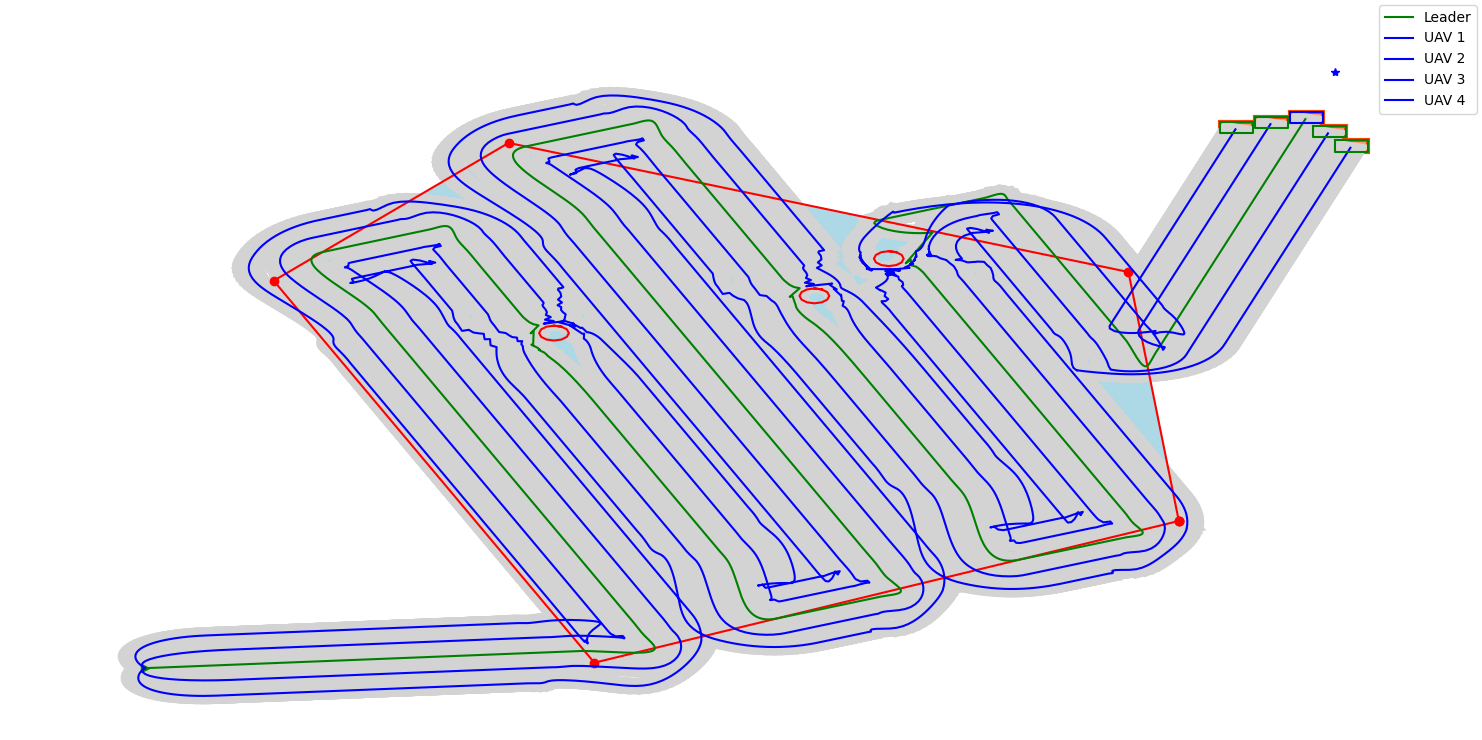
\includegraphics[width=\textwidth]{chapter5/image/obs.png}
    \caption{}
    \label{fig:obs}
    \end{subfigure}
    %\hspace{-0.5cm}
    \begin{subfigure}[b]{0.49\textwidth}
    \centering 
    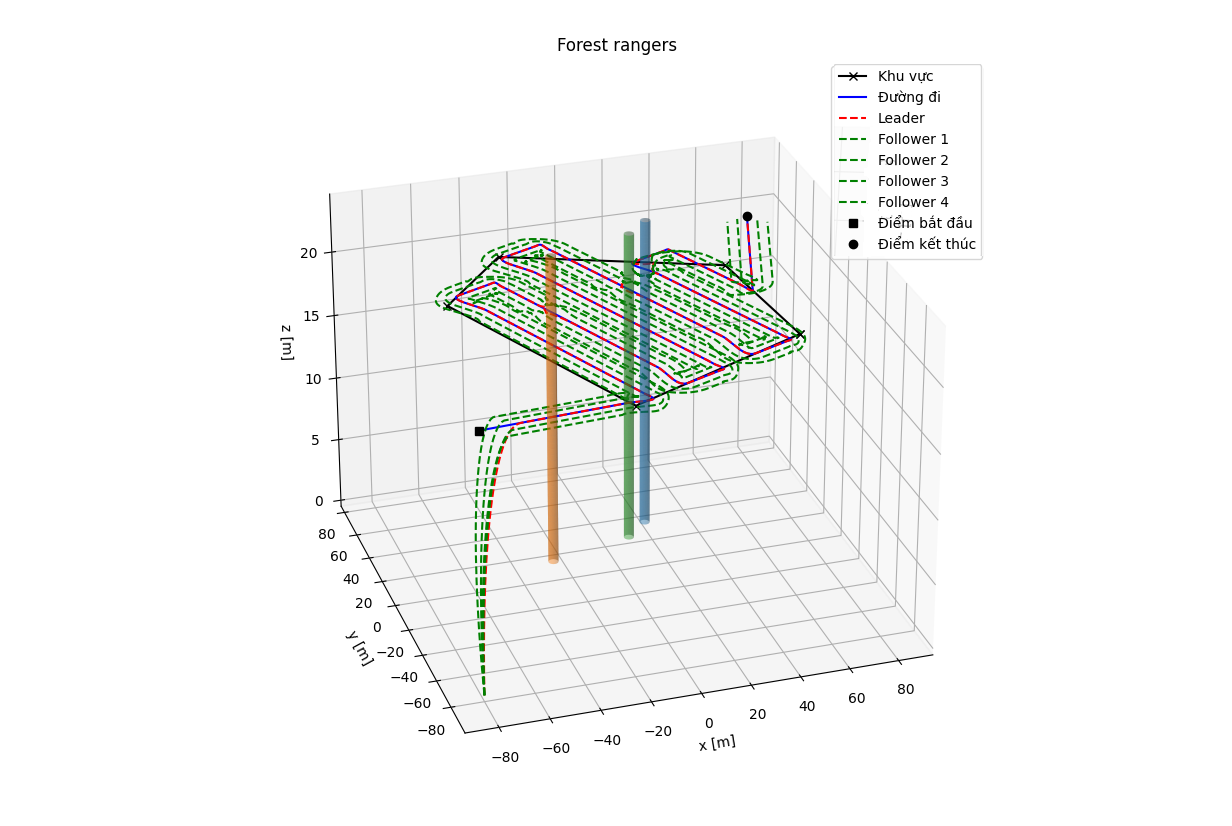
\includegraphics[width=\textwidth]{chapter5/image/obs3d.png}
    \caption{}
    \label{fig:obs3d}
    \end{subfigure}
    \caption{Quá trình di chuyển tránh chướng ngại vật của đội hình chữ V }
    \label{fig:5Robots}
\end{figure}

\begin{figure}[H]
    \centering
    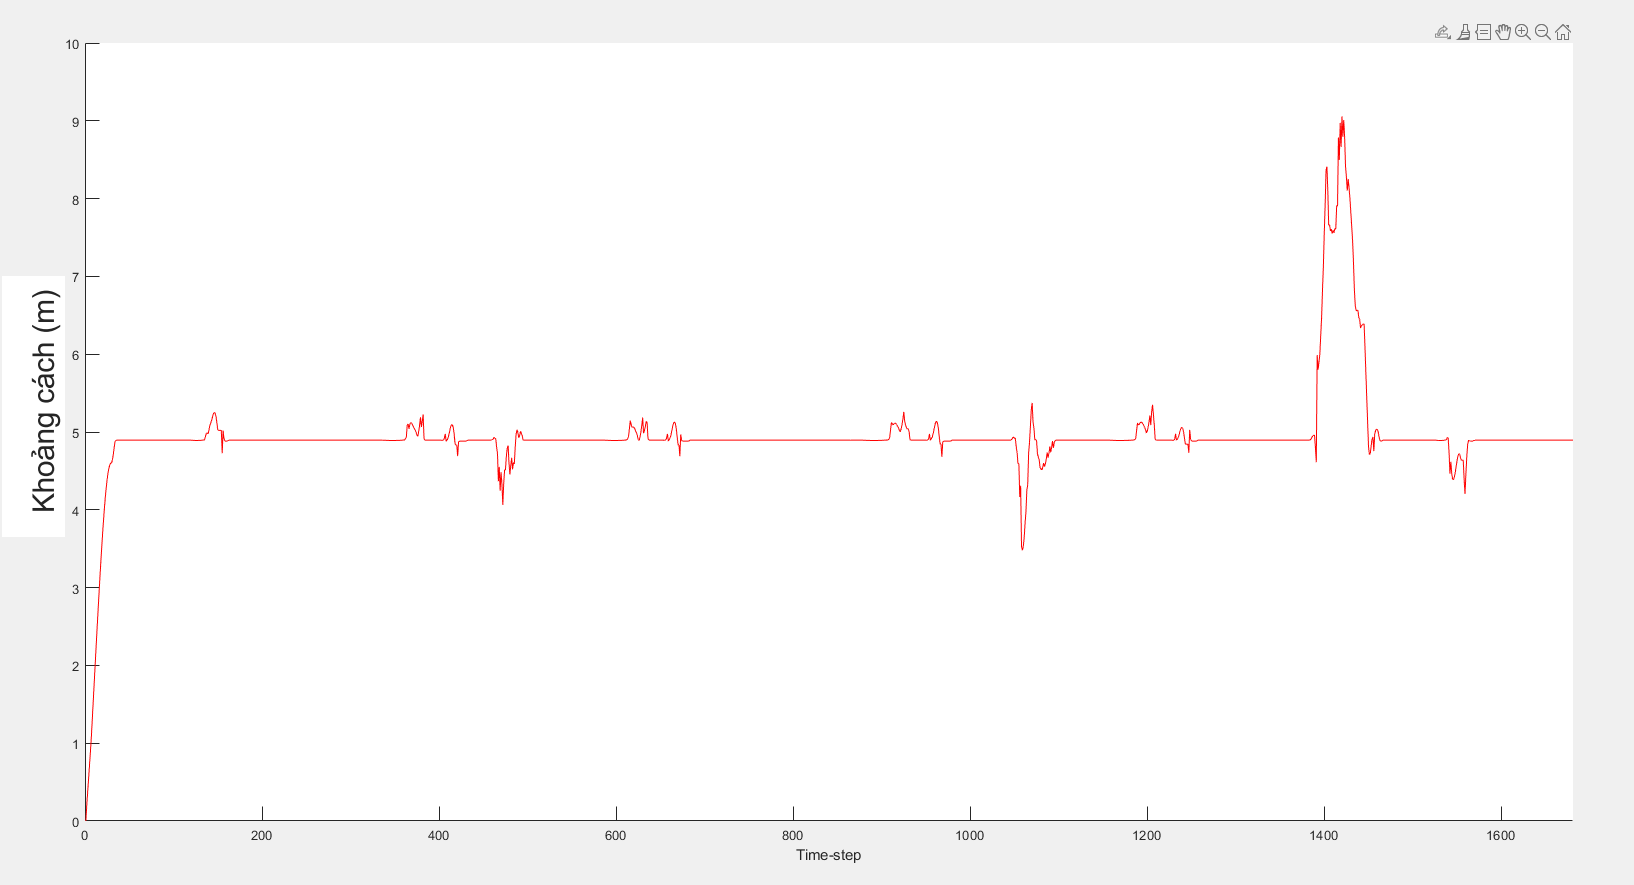
\includegraphics[width=0.8\textwidth]{chapter5/image/poserrobs.png}
    \caption{Khoảng cách trung vị giữa 2 con robot liên tiếp}
    \label{fig:poserrobs}
\end{figure}
Hình \ref{fig:obs} cho thấy được quỹ đạo của các robot trong quá trình di chuyển gặp chướng ngại vật. Các robot đã chủ động tránh vật cản trên đường đi của chúng. Tuy nhiên điều đó đã gây ra sự xáo trộn trong đội hình đặc biệt là khi vật cản ở ngay góc cua sẽ gây ra sự đột biến lớn trong quỹ đạo di chuyển của Leader. Điều này càng được chỉ ra rõ hơn ở trong Hình \ref{fig:poserrobs} khi tránh vật cản, thì khoảng cách trung vị giữa 2 robot liên tiếp không còn được giữ ổn định nữa. Lúc này đã gây ra sự xáo trộn ở trong đội hình. Đặc biệt khi tránh chướng ngại vật thứ 3 ở ngay khúc cua, leader thực sự đã lệch một khoảng cách rất lớn so với quỹ đạo đưa ra. Tuy nhiên nhờ có hành vi giữ đội hình mà đội hình di chuyển dần dần ổn định trở lại và tiếp tục quét các vùng còn lại. Ngoài ra Hình \ref{fig:obs} cũng cho thấy khi quét qua chướng ngại vật thì một phần vùng xung quanh chướng ngại vật không thể bị quét qua, làm giảm hiệu suất bao phủ xuống 91.88$\%$. Tuy nhiên điều này có thể chấp nhận được vì, robot bắt buộc phải thực hiện hành vi tránh vật cản để không gây ảnh hưởng đến đội hình.

Tổng kết, thuật toán tối ưu đường đi bao phủ được đề xuất đã đạt kết quả cao trong cả tỉ lệ quét bao phủ và thời gian bay. Việc sử dụng Op-RCPP để thiết kế đường đi bao phủ khi dùng với nhiều robot thì phù hợp hơn sử dụng phương pháp chia lưới.

\nocite{*}
\renewcommand{\bibname}{References}
\printbibliography
\addcontentsline{toc}{chapter}{References}

\end{document}